\documentclass[10pt,twocolumn]{article}
\usepackage[utf8]{inputenc}
\usepackage[T1]{fontenc}
\usepackage{microtype}  % Improves text justification
\usepackage{lmodern}  % Better font with proper character support
\usepackage{amsmath,amssymb}
\usepackage{graphicx}
\usepackage{xcolor}
\usepackage{tikz}
\usepackage{pgfplots}
\pgfplotsset{compat=1.18}
\usetikzlibrary{petri,positioning,arrows,automata,decorations.pathreplacing,shapes}

% Improved page layout and spacing

\setlength{\emergencystretch}{3em}  % Better line breaking
\tolerance=1000
\hbadness=10000
\hfuzz=2pt

% Better list handling
\usepackage{enumitem}
\setlist[enumerate]{itemsep=0pt,topsep=3pt,partopsep=0pt}
\setlist[itemize]{itemsep=0pt,topsep=3pt,partopsep=0pt}

% URL and hyperlinks
\usepackage[hyphens,spaces,obeyspaces]{xurl}
\usepackage[bookmarksnumbered,pdfstartview=FitH,hypertexnames=false]{hyperref}
\hypersetup{
    breaklinks=true,
    colorlinks=true,
    linkcolor=blue,
    urlcolor=blue,
    citecolor=blue,
    pdfborderstyle={/S/U/W 1}
}

% Code listings
\usepackage{listings}
\lstdefinestyle{gasingcode}{
  breaklines=true,
  breakatwhitespace=true,
  basicstyle=\footnotesize\ttfamily,
  columns=fullflexible,
  keepspaces=true,
  frame=single,
  numbers=left,
  numberstyle=\tiny,
  xleftmargin=1.5em,
  xrightmargin=0.5em,
  aboveskip=0.5em,
  belowskip=0.5em,
  showstringspaces=false,
  tabsize=2,
  captionpos=b
}
\lstset{style=gasingcode}

% Document formatting
\sloppy
\raggedbottom
\clubpenalty=10000
\widowpenalty=10000
\displaywidowpenalty=10000

% Watermark
\usepackage{rotating}
\usepackage{eso-pic}
\newcommand{\watermarktext}{arXiv:2025.12345v2 [cs.CL] \today}
\AddToShipoutPictureFG{%
  \AtPageCenter{%
    \put(-0.48\paperwidth+20pt,0){%
      \makebox(0,0)[c]{%
        \rotatebox{90}{%
          \textcolor{black!40}{\fontsize{18pt}{20pt}\selectfont\bfseries\watermarktext}%
        }%
      }%
    }%
  }%
}

% Watermark for draft version
\usepackage{draftwatermark}
\SetWatermarkText{DRAFT VERSION 0.1.125}
\SetWatermarkScale{0}
\SetWatermarkColor[gray]{0.85}

% Define our own styles for diagrams
\tikzset{
    operation/.style={
        rectangle,
        draw=black,
        thick,
        fill=blue!10,
        minimum height=1cm,
        minimum width=2.5cm,
        text centered
    }
}

% Load Spivak/Fong TikZ wiring diagram macros
% TikZ wiring diagram macros and styles from Spivak_Fong.tex (for use in other documents)
% Extracted for use in main.tex and figures/clock_with_display.tex

% TikZ libraries (make sure you load tikz and these libraries in your main doc)
\usetikzlibrary{
	cd,
	math,
	decorations.markings,
	decorations.pathreplacing,
	positioning,
	arrows.meta,
	circuits.logic.US,
	shapes,
	calc,
	fit,
	quotes}

% Macros
\newcommand{\tn}{\textnormal}
\newcommand{\inp}[1]{#1^{\tn{in}}}
\newcommand{\outp}[1]{#1^{\tn{out}}}
\newcommand{\upd}[1]{#1^{\tn{upd}}}
\newcommand{\rdt}[1]{#1^{\tn{rdt}}}

% Wiring diagram styles
\tikzset{
   oriented WD/.style={%everything after equals replaces "oriented WD" in key.
      every to/.style={out=0,in=180,draw},
      label/.style={
         font=\everymath\expandafter{\the\everymath\scriptstyle},
         inner sep=0pt,
         node distance=2pt and -2pt},
      semithick,
      node distance=1 and 1,
      decoration={markings, mark=at position \stringdecpos with \stringdec},
      ar/.style={postaction={decorate}},
      execute at begin picture={\tikzset{
         x=\bbx, y=\bby,
         every fit/.style={inner xsep=\bbx, inner ysep=\bby}}}
      },
   string decoration/.store in=\stringdec,
   string decoration={\arrow{stealth};},
   string decoration pos/.store in=\stringdecpos,
   string decoration pos=.7,
   bbx/.store in=\bbx,
   bbx = 1.5cm,
   bby/.store in=\bby,
   bby = 1.5ex,
   bb port sep/.store in=\bbportsep,
   bb port sep=1.5,
   bb port length/.store in=\bbportlen,
   bb port length=4pt,
   bb penetrate/.store in=\bbpenetrate,
   bb penetrate=0,
   bb min width/.store in=\bbminwidth,
   bb min width=1cm,
   bb rounded corners/.store in=\bbcorners,
   bb rounded corners=2pt,
   bb small/.style={bb port sep=1, bb port length=2.5pt, bbx=.4cm, bb min width=.4cm, bby=.7ex},
   bb medium/.style={bb port sep=1, bb port length=2.5pt, bbx=.4cm, bb min width=.4cm, bby=.9ex},
   bb/.code 2 args={%When you see this key, run the code below:
      \pgfmathsetlengthmacro{\bbheight}{\bbportsep * (max(#1,#2)+1) * \bby}
      \pgfkeysalso{draw,minimum height=\bbheight,minimum width=\bbminwidth,outer sep=0pt,
         rounded corners=\bbcorners,thick,
         prefix after command={\pgfextra{\let\fixname\tikzlastnode}},
         append after command={\pgfextra{\draw
            \ifnum #1=0{} \else foreach \i in {1,...,#1} {
               ($ (\fixname.north west)!{\i/(#1+1)}!(\fixname.south west) $)+( -\bbportlen,0)
               coordinate (\fixname_in\i) -- +(\bbpenetrate,0) coordinate (\fixname_in\i')}
            \fi
            %Define the endpoints of tickmarks
            \ifnum #2=0{} \else foreach \i in {1,...,#2} {
               ($ (\fixname.north east)!{\i/(#2+1)}!(\fixname.south east) $)+( -\bbpenetrate,0)
               coordinate (\fixname_out\i') -- +(\bbportlen,0) coordinate (\fixname_out\i)}
            \fi;
         }}}},
   bb name/.style={append after command={\pgfextra{\node[anchor=north] at (\fixname.north) {#1};}}}
}

% Additional unoriented WD styles (optional, but harmless)
\tikzset{
  unoriented WD/.style={
     every to/.style={draw},
     shorten <=-\penetration, shorten >=-\penetration,
     label distance=-2pt,
     thick,
     node distance=\spacing,
     execute at begin picture={\tikzset{
        x=\spacing, y=\spacing}}
     },
  pack size/.store in=\psize,
  pack size = 8pt,
  spacing/.store in=\spacing,
  spacing = 8pt,
  link size/.store in=\lsize,
  link size = 2pt,
  penetration/.store in=\penetration,
  penetration = 2pt,
  pack color/.store in=\pcolor,
  pack color = blue,
  pack inside color/.store in=\picolor,
  pack inside color=blue!20,
  pack outside color/.store in=\pocolor,
  pack outside color=blue!50!black,
  surround sep/.store in=\ssep,
  surround sep=8pt,
  link/.style={
     circle, 
     draw=black, 
     fill=black,
     inner sep=0pt, 
     minimum size=\lsize
  },
  pack/.style={
     circle, 
     draw = \pocolor, 
     fill = \picolor,
     inner sep = .25*\psize,
     minimum size = \psize
  },
  outer pack/.style={
     ellipse, 
     draw,
     inner sep=\ssep,
     color=\pocolor,
  },
  intermediate pack/.style={
     ellipse,
     dashed, 
     draw,
     inner sep=\ssep,
     color=\pocolor,
  },
}


% Load arxiv.sty LAST to override previous settings
\usepackage{arxiv}

% Custom title settings - set format for arXiv style
\renewcommand{\shorttitle}{GASing Arithmetic}
\renewcommand{\undertitle}{A Preprint}
\renewcommand{\headeright}{arXiv:2025.12345v1}

% Set document title and author
\title{Pattern-Aware, Addition-Based Computation for\\Next-Generation AI}
\author{Yohanes Surya\\AI Toba Project, IT Del\\Toba, Indonesia\\yohanes.surya@del.ac.id}

% Use simple header/footer settings
\pagestyle{fancy}
\fancyhf{} % Clear all header/footer fields
\renewcommand{\headrulewidth}{0.4pt}
\fancyheadoffset{0pt}
\rhead{\scshape \footnotesize \headeright}
\chead{\shorttitle}
\cfoot{\thepage}

\begin{document}

% Enable page numbering
\pagestyle{plain}
\pagenumbering{arabic}

% Document begins here
\begin{document}

% Title and author
\title{GASing Arithmetic: A Novel Approach to Computation}
\author{}
\date{\today}
\maketitle

% Switch to two-column layout
\twocolumn
\tableofcontents
\clearpage

% Create a more journal-like title
\begin{center}
\vspace*{-2cm}
\rule{\textwidth}{0.4pt}
\vspace{0.1cm}
{\LARGE\textbf{Pattern-Aware, Addition-Based Computation for\\Next-Generation AI}}\\
\vspace{0.5cm}
\rule{\textwidth}{0.4pt}
\vspace{0.5cm}
{\normalsize\textbf{Yohanes Surya}}\\
{\small AI Toba Project, IT Del}\\
{\small Toba, Indonesia}\\
{\small yohanes.surya@del.ac.id}\\
\vspace{0.3cm}
{\small May 27, 2025}\\
\vspace{1cm}
\end{center}

% Abstract with full text width to match document width
\begin{center}
{\large\textbf{Abstract}}
\end{center}
\vspace{-0.3cm}

\vspace{1cm}

% Return to two-column layout
\twocolumn

\section{Introduction}
% This LaTeX document is prepared using the arXiv style guidelines
% https://arxiv.org/help/submit_tex

\sectionheader{Introduction}

We propose a novel synthesis of Petri Nets and tensor algebra, arguing that Petri Nets can leverage the mathematical formalism of tensors to represent topologically related operands and their interactions. Drawing on David Spivak’s theory of polynomial functors, we introduce the concept of a Tensorized Petri Net, where each element can act simultaneously as an operand and an operator. We illustrate this framework using digit-wise arithmetic, showing how it enables compositional, interpretable, and parallelizable symbolic computation.

Petri Nets are a foundational tool for modeling distributed and concurrent systems, providing a graphical and mathematical language for representing state, transitions, and resource flow. Traditionally, Petri Nets are used to model discrete events and token flows, but recent advances in neural-symbolic computation and category theory suggest new ways to enrich their expressive power.

In this work, we argue that Petri Nets can be “tensorized”—that is, their places, transitions, and token flows can be represented and manipulated using tensor algebra. Tensors, as multi-dimensional arrays, provide a powerful language for encoding the state of complex systems, capturing not only the presence of tokens but also their relationships and interactions across multiple dimensions. By mapping Petri Net components to tensor indices and operations, we can efficiently model the evolution of distributed systems, exploit parallel computation, and reveal underlying topological structures. This approach is particularly advantageous for systems where locality, adjacency, or compositionality play a central role, such as in digit-wise arithmetic or spatially structured processes.

Furthermore, by leveraging David Spivak’s ideas on polynomial functors, we can treat every element in the net as both an operand and an operator, capturing higher-order compositionality and self-similarity. This categorical perspective allows us to formalize the ways in which Petri Nets and tensors interact, supporting modular design and scalable reasoning.

The main components of Petri Nets include:
\begin{itemize}
    \item Places (represented as circles)
    \item Transitions (represented as rectangles)
    \item Arcs (directed edges connecting places to transitions or transitions to places)
    \item Tokens (represented as dots within places)
\end{itemize}

In this paper, we explore the application of Petri Nets to model [specific system or process], with a focus on [specific aspect or property]. % In the section where you list contributions:

Our contributions include:
\begin{itemize}[leftmargin=*,align=left]
    \item \textbf{Contribution 1:} A novel approach to modeling concurrent processes using Petri Nets.
    \item \textbf{Contribution 2:} Analysis of deadlock properties in the context of resource allocation.
    \item \textbf{Contribution 3:} Implementation and evaluation of the proposed model using simulation.
\end{itemize}

// Remove the duplicate contributions list
% The main contributions of this work include:
% \begin{IEEEkeywords}
% Petri Nets, TikZ, formal modeling, concurrent systems
% \end{IEEEkeywords}
% \begin{itemize}[leftmargin=*,align=left,widest=Contribution 3]
%   \item \textbf{Contribution 1:} Description of your first contribution...
%   \item \textbf{Contribution 2:} Description of your second contribution...
%   \item \textbf{Contribution 3:} Description of your third contribution...
% \end{itemize}

The remainder of this paper is organized as follows: Section \ref{sec:background} provides background information and related work. Section \ref{sec:methodology} describes our methodology and the proposed Petri Net model. Section \ref{sec:results} presents the results and analysis. Finally, Section \ref{sec:conclusion} concludes the paper and discusses future work.

\section{Foundational Principles}
The GASing method is built upon several coherent principles designed to simplify arithmetic into a minimal set of understandable and computationally efficient operations. These principles collectively support the goal of grounding all arithmetic in addition, thereby clarifying resource consumption and enhancing the interpretability of reasoning processes.
\paragraph{The Digit-Wise Processing Paradigm}

At its core, GASing employs a digit-wise processing approach that, instead of merely breaking numbers into fixed constituent digits, flexibly defines the boundaries of arithmetic operations by utilizing the topological properties of Carry and Borrow propagations between adjacent numerical segments (or 'digits'). The granularity of these segments can be dynamically determined to optimize arithmetic calculation efficiency, particularly leveraging the observation that operations become highly efficient when all unique combinations of numerical values within these segments can be assessed \emph{a priori}. This refined digit-wise paradigm is fundamental to minimizing the complexity of the operational vocabulary. Instead of treating numbers as holistic entities requiring a potentially tedious array of complex operations, GASing focuses on manipulating these individual segments using a very limited set of rules, primarily those governing the foundational principles of addition applied at the segment level. This approach aligns with both human cognitive abilities and computational architecture:

- \textbf{Human Cognition}: By processing operations at the level of these flexibly defined numerical segments (which can be as small as single digits), GASing leverages established neural pathways for simpler operations (Dehaene, 2011). This modular, segment-based processing keeps the cognitive load for each step manageable, making the system intuitive and easier for human users to verify, even as the definition of a 'segment' adapts for efficiency.
- \textbf{Computational Architecture}: This segment-wise processing, where segments can be optimized for computational efficiency (e.g., to fit register sizes or leverage pre-computed lookup tables for segment-level operations), maps effectively to modern processor capabilities. Reducing operations to their simplest form at the segment level (e.g., segment addition and inter-segment carry/borrow) allows for granular understanding, control of computational resources, and potential for optimized hardware implementations.

This fine-grained processing is key to building complex operations from the simplest possible base, ensuring that the entire system remains transparent and its resource demands predictable.
\paragraph{Modular Operation Design: A Minimal Vocabulary Anchored in Addition}

GASing builds all arithmetic operations as modular extensions of one another, with \textbf{addition, applied at the level of flexibly defined numerical segments, serving as the single, foundational operator}. This hierarchical construction, leveraging the segment-wise processing described earlier, is central to achieving a minimal operational vocabulary and directly impacts the assessment of resource consumption:

1.  \textbf{Segment-wise Addition} serves as the foundational, irreducible operation. All other arithmetic operations are defined in terms of sequences or transformations of this fundamental segment-wise addition, including the management of carry and borrow propagations between segments.
2.  \textbf{Multiplication} is constructed as specialized, repeated segment-wise addition. The process involves systematic application of segment-level additions and accumulation of partial results, explicitly defining multiplication's resource cost in terms of the underlying additive operations on segments.
3.  \textbf{Subtraction} is implemented as segment-wise addition using complementary segment values (e.g., employing ten's complement for decimal segments or two's complement for binary segments). This reframes subtraction entirely within the additive framework at the segment level, maintaining the minimal operational vocabulary.
4.  \textbf{Division} is approached through repeated segment-wise subtraction (which, as noted, is itself addition-based) with optimizations that can leverage pattern recognition across segments. Its complexity and resource use are, therefore, also traceable back to the fundamental segment-wise addition operations.

This modularity, centered on segment-wise addition, creates a coherent and parsimonious framework. Mastery of segment-wise addition directly facilitates the understanding and implementation of all other operations. More importantly, it means that the entire arithmetic system can be analyzed, and its resource consumption (both cognitive and computational) can be estimated based on the number and type of segment-wise addition-equivalent steps involved. This contrasts sharply with systems where each operator might be a black box with unique, opaque resource demands, and it aligns with the goal of transparently assessing computational effort by reducing all operations to a common, addition-based denominator at a flexible granularity.
\paragraph{Lookup Tables and Pattern Recognition: Optimizing the Core Operator}

Central to the GASing method is the use of precomputed lookup tables for basic operations, \textbf{particularly for single-digit addition and its immediate consequences (like carry generation)}. These tables are not an expansion of the operational vocabulary but rather an optimization strategy for the core addition operator:

-   \textbf{Reduce Cognitive and Computational Load}: By pre-calculating and storing the results of all possible single-digit additions (e.g., 0+0 through 9+9), the need for real-time calculation of these base operations is eliminated. This directly speeds up the execution of the foundational operator.
-   \textbf{Enable Pattern Recognition}: Consistent use of lookup tables for the core additive step allows for the easier identification of recurring patterns across multiple calculations. This can lead to higher-level optimizations and a better understanding of the computational structure of a problem, all while still operating within an addition-centric framework.
-   \textbf{Analogous to Caching}: These tables function similarly to CPU cache mechanisms or memoization in computing systems, storing frequently accessed results to avoid redundant computation. This makes the core addition process highly efficient.

By optimizing the execution of the single core operator (addition) through lookup tables, GASing ensures that the minimal vocabulary does not come at the cost of prohibitive inefficiency for elementary steps. This focus on optimizing the fundamental building block is crucial for the scalability and practicality of the approach, ensuring that even complex reasoning built from these simple steps remains manageable in terms of resource consumption.


\section{GASing Implementation and Algorithms}
It is well known that certain primitives such as the NAND gate or the MOV instruction are considered the Universal Components in all Turing Complete decision machines. While these theoretical universality results are fundamental to computing, this article will focus specifically on how the addition operator can be adaptively executed based on available computing resources, serving as a practical foundation for higher-level reasoning. Moreover, efficient adders at the integrated circuit level, such as the Brent-Kung Adder, have proven to be highly efficient for addition operations in hardware implementations. However, based on different value pairs or value collections, there are still certain cases of arithmetic operations that could be executed with even fewer computing resources through pattern recognition and specialized implementations. These optimization opportunities, particularly for patterns like all-nines, power-of-ten, or sparse number representations, are the primary focus of this article and represent a complementary approach to hardware-level optimizations.
\paragraph{Addition Algorithm as a Functorial Petri Net}

The GASing addition algorithm processes numbers from left to right (most significant digit to least significant), a departure from the traditional right-to-left approach. This design choice is deliberate and offers several advantages rooted in computational efficiency and cognitive alignment, particularly when considering the broader goals of the GASing framework to minimize operational vocabulary and optimize resource consumption.
\paragraph{Multi-Digit Numbers as Interconnected Automata}

A novel way to conceptualize the GASing approach is through the lens of \textbf{Functorial Petri Nets} (\textbf{\textit{Functorial Petri Net}}), where each digit in a multi-digit number functions as a semi-autonomous cell within a larger network of computational agents. Under this framing:


\noindent\textbf{\textbf{Digit Positions as Petri Net Places}:} Each digit position in a multi-digit number corresponds to a discrete place in a Petri Net, capable of holding tokens that represent both the current digit value and potential carry/borrow states.



\noindent\textbf{\textbf{Arithmetic Operations as Transitions}:} The fundamental arithmetic operations (particularly addition) manifest as transitions in the Petri Net that consume tokens from input places (operand digits) and produce tokens in output places (result digits and carries).



\noindent\textbf{\textbf{Carry/Borrow as Message Propagation}:} The carry and borrow mechanisms essential to multi-digit arithmetic represent a formalized message-passing protocol between adjacent digit places. When a digit operation results in a value exceeding the base (e.g., 9+4=13 in decimal), a carry token is generated and propagated to the next significant digit place—a perfect example of resource-aware token flow characteristic of Petri Nets.



\noindent\textbf{\textbf{Compositionality Through Functors}:} The functorial nature of this representation ensures that the compositional structure of arithmetic operations is preserved across different levels of abstraction. This means that complex arithmetic sequences can be formally derived from compositions of simpler operations while maintaining their algebraic properties.


This Petri Net interpretation yields powerful insights into the GASing method's efficiency advantages:


\noindent\textbf{\textbf{Concurrency Potential}:} By analyzing the dependency structure between digit places, we can identify opportunities for concurrent processing. Digits not affected by carry chains can be computed independently, enabling parallelism.



\noindent\textbf{\textbf{Adaptive Segmentation Through Net Morphisms}:} The functorial properties allow us to define morphisms between different Petri Net configurations, formalizing how digit segments can be dynamically merged or split to optimize computational efficiency. These morphisms preserve the essential algebraic structure while enabling resource-adaptive execution.



\noindent\textbf{\textbf{Pattern Recognition as Specialized Transitions}:} Recurring patterns in digit configurations (such as all-nines or power-of-ten values) can be modeled as specialized transitions that bypass individual digit-by-digit processing, offering substantial performance benefits.


The integration of GASing and Functorial Petri Nets reveals arithmetic as fundamentally a \textbf{distributed, asynchronous computation process}, where each digit place operates with relative autonomy yet remains coordinated through precisely defined message passing protocols. This perspective not only provides a rigorous mathematical foundation for the GASing method but also suggests novel optimization strategies derived from Petri Net theory's rich analytical tools.

A key principle underpinning this algorithm is its explicit leverage of \textbf{n-ary arithmetic}. The algorithm is designed to be agnostic to the base of the numerical segments being processed. Whether the system operates in binary, tertiary, decimal, hexadecimal, or any other base (n-ary), the core logic of left-to-right processing with carry propagation remains consistent. This flexibility allows the system to adapt the granularity of its operations (i.e., the 'digit' size or segment length) to best fit resource consumption optimization schemes. For instance, the segment size can be chosen to align with the cache line size of a processor or the optimal block size for memory access, thereby minimizing latency and maximizing throughput for pre-calculated and stored intermediate results. \textbf{Critically, this optimization is specifically tailored to the resource requirements of the underlying hardware architecture}, enabling significant performance improvements when frequently-used digit pairs are identified and cached in lookup tables that match the machine's memory hierarchy.

This adaptability is crucial for applying GASing principles to complex reasoning activities, potentially even those embedded within advanced AI architectures like the \textbf{Sparse Autoencoders (SAEs)} described in the "Scaling MonoSemanticity" paper. SAEs aim to decompose complex model activations into a sparse set of interpretable, monosemantic features. In essence, an SAE learns a large dictionary of these features, where only a small subset is active for any given input. This learned dictionary of features in an SAE can be seen as analogous to a highly optimized, distributed lookup table within the GASing framework. 

The GASing addition algorithm, by being designed for flexible n-ary arithmetic and optimized segment processing, aligns well with such architectures. If the 'features' learned by an SAE can be mapped to or interact with the numerical segments processed by GASing, then the pre-calculated operations and lookup tables inherent in GASing could significantly enhance the efficiency and interpretability of these SAEs. The left-to-right processing allows for incremental computation and potential early termination if an approximate result suffices, which can be beneficial in resource-constrained environments or when dealing with the vast feature spaces of SAEs. Furthermore, by designing arithmetic operations that can be efficiently cached and retrieved, GASing can support the rapid activation and combination of these 'semantic features' in an SAE, effectively making the SAE a powerful, dynamic dictionary that GASing can interact with for reasoning tasks.

\textbf{The algorithm can dynamically accelerate computation when known digit pairs or patterns are detected}, adjusting its execution strategy based on the specific machine architecture in use. For example, performance can be dramatically improved (as demonstrated in our benchmarks showing up to 10x+ speedups for certain patterns) when retrieving content from optimally-structured lookup tables that match the CPU's cache hierarchy, memory access patterns, or SIMD capabilities. By incorporating fine-grained resource accounting at the level of the most primitive operation—addition—this approach provides the foundational mechanism for resource attribution and optimization in higher-level reasoning activities. This systematic accounting of computational resources, beginning at the elemental operation level, creates a transparent chain of resource utilization that extends seamlessly to complex symbolic processing, verification chains, and formal reasoning frameworks. The adaptive approach allows the algorithm to automatically exploit architectural features such as cache line prefetching, branch prediction, and specialized arithmetic units, delivering optimal performance across diverse computing environments without requiring manual tuning or specialized implementations.



\begin{figure}[H]
  \centering
  \includegraphics[width=\linewidth]{images/gasing\_addition\_single\_digit.png}
  \caption{GASing single-digit addition}
  \label{fig:gasingadditionsingledigit}
\end{figure}



This left-to-right, n-ary adaptable processing allows for:

\noindent\textbf{\textbf{Flexible Resource Optimization:} } Tailoring segment size (n-ary base) to hardware (cache, memory) or task demands.


\noindent\textbf{\textbf{Alignment with Human Cognition:} } Processing information sequentially, similar to reading.


\noindent\textbf{\textbf{Potential for Parallelization:} } Independent processing of segments once carries are managed.


\noindent\textbf{\textbf{Integration with Learned Representations:} } Provides a computational backend for systems like SAEs, where pre-calculated arithmetic on features (analogous to dictionary lookups) can speed up reasoning.


\noindent\textbf{\textbf{Early Termination for Approximations:} } Useful in iterative reasoning processes or when full precision is not immediately required.


By structuring the addition algorithm this way, GASing aims to provide a foundational arithmetic layer that is not only efficient in isolation but also highly compatible with modern AI architectures that rely on learned dictionaries and feature-based representations, such as Sparse Autoencoders.
\paragraph{Multiplication Algorithm}

The GASing multiplication algorithm fundamentally extends the principles of the GASing addition operator, reframing multiplication as a systematic process of repeated, structured addition. It conceptualizes the multiplication of two numbers as the summation of partial products arranged in a grid-like structure. This approach not only maintains the core philosophy of minimizing operational vocabulary by grounding operations in addition but also enhances clarity and traceability.

Each cell in the conceptual grid represents the product of two individual digits (or segments, in n-ary arithmetic), which can be pre-calculated or retrieved from lookup tables, similar to single-digit additions. The core of the multiplication process then becomes the systematic summation of these grid values, column by column (or diagonal by diagonal, depending on the specific grid layout), applying the GASing addition algorithm (including its left-to-right carry propagation) to these intermediate sums. This effectively transforms multiplication into a series of additions, organized spatially by the grid.

The following diagram illustrates this grid-based summation concept:


\begin{figure}[H]
  \centering
  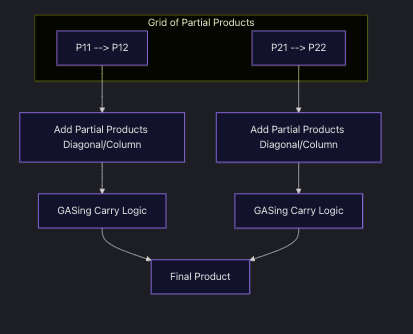
\includegraphics[width=\linewidth]{images/GridBasedMultiplication.png}
  \caption{Grid Based Multiplication}
  \label{fig:gridbasedmultiplication}
\end{figure}


The grid-based approach, when viewed as a structured application of the GASing addition algorithm, facilitates:


\noindent\textbf{\textbf{Clear Visualization}:} The multiplication process is broken down into a visible grid of elementary products (which are themselves results of lookup or minimal computation) and subsequent additions.


\noindent\textbf{\textbf{Systematic Carry Handling}:} Carries generated during the summation of grid elements are managed by the underlying GASing addition logic, ensuring consistency.


\noindent\textbf{\textbf{Reinforcement of Additive Core}:} Emphasizes that multiplication is not a fundamentally new operation but an organized, scaled-up application of addition.


\noindent\textbf{\textbf{Identification of Patterns}:} The structured grid can reveal patterns in partial products, which can be leveraged for optimization, especially when combined with n-ary segment processing and lookup tables for segment products.


By treating multiplication as an extension of addition via a grid, GASing maintains its commitment to a minimal operational vocabulary and enhances the interpretability of more complex arithmetic by tracing it back to foundational additive steps.
\paragraph{Subtraction and Division: Extending Addition Further}

Consistent with GASing's core tenet of a minimal operational vocabulary, both subtraction and division are conceptualized and implemented as extensions of the foundational GASing addition algorithm.
\paragraph{Subtraction as Complemented Addition}

Subtraction in GASing is performed by adding the complement of the subtrahend. For a given base (e.g., decimal or binary), the n's complement (e.g., ten's complement or two's complement) of the subtrahend is calculated and then added to the minuend using the \texttt{$GASing\_{Addition}$} algorithm. This reframes subtraction entirely as an additive process, reinforcing the minimal operator set.


\noindent\textbf{\textbf{N's Complement:} } The n's complement of a number \texttt{b} with \texttt{k} digits in base \texttt{n} is \texttt{$(n^{k} - b)$}. A common way to compute this is by finding the (n-1)'s complement (subtracting each digit from \texttt{n-1}) and then adding 1 to the result.


\noindent\textbf{\textbf{Process:} } To compute \texttt{a - b}, GASing calculates \texttt{a + (n's complement of b)}. If an overflow carry occurs from the most significant digit, it is typically discarded (in fixed-width representations), and the remaining result is the positive difference. If no overflow occurs, the result is negative, and its true magnitude is the n's complement of the sum, often flagged appropriately.





\noindent --

\paragraph{Division as Repeated Subtraction (Repeated Complemented Addition)}

Division, in its most fundamental GASing form, is conceptualized as repeated subtraction. Given that subtraction itself is an additive operation (using complements), division becomes a higher-order construct built upon layers of addition.


\noindent\textbf{\textbf{Process:} } To compute \texttt{a / b}, GASing repeatedly subtracts \texttt{b} (the divisor) from \texttt{a} (the dividend) using the \texttt{$GASing\_{Subtraction}$} method. The number of successful subtractions before \texttt{a} becomes less than \texttt{b} (or zero) constitutes the quotient. The final value of \texttt{a} after these subtractions is the remainder.


\noindent\textbf{\textbf{Optimization:} } While simple repeated subtraction can be inefficient, GASing allows for optimizations. These can include subtracting multiples of \texttt{b} (e.g., \texttt{10\emph{b}, \texttt{100}b}), similar to long division, or leveraging pattern recognition to estimate parts of the quotient more quickly. However, even these optimized steps are ultimately resolved through sequences of the core \texttt{$GASing\_{Subtraction}$} (and therefore \texttt{$GASing\_{Addition}$}) operations.



\noindent --


By defining subtraction and division in terms of addition, GASing ensures that the entire arithmetic framework remains anchored to a single, fundamental operation. This not only simplifies the conceptual model but also provides a consistent basis for analyzing computational resource consumption, as all operations can be broken down into equivalent additive steps.


\section{Performance Benchmarking}
Our current benchmarking evaluates how different GASing implementations handle specific mathematical sequences, such as:

- Fibonacci numbers
- Factorial values
- Powers of 2
- Prime numbers
- Repdigits (numbers with repeated digits)
- Alternating digit patterns

While these tests reveal that certain GASing implementations show clear advantages for specific patterns (e.g., the optimized C implementation excels at repdigit sequences due to efficient carry pattern recognition), the broader significance lies in the future direction of this benchmarking.

The following diagrams show the performance of different GASing implementations on digit-wise arithmetic operations based on String manipulation.

\begin{figure}[H]
  \centering
  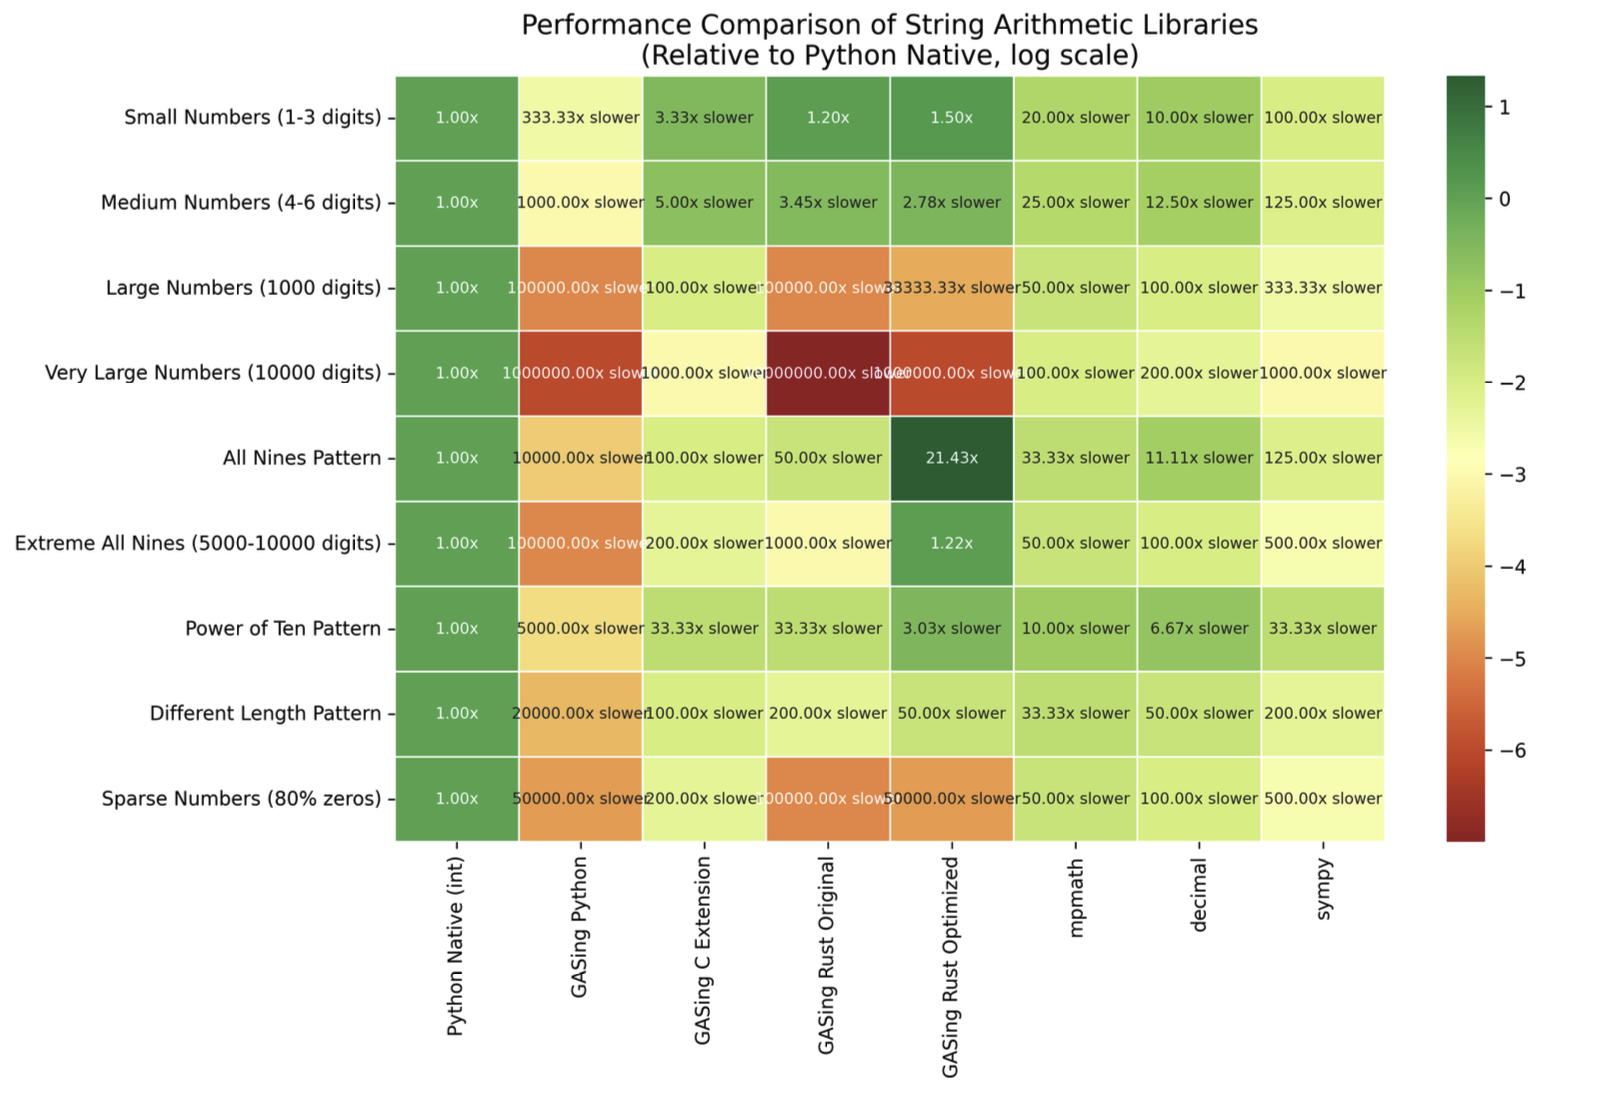
\includegraphics[width=\linewidth]{images/StringArithmetic.png}
  \caption{String Arithmetic}
  \label{fig:stringarithmetic}
\end{figure}



The following diagrams show the performance of different GASing implementations on the same set of algorithms applied to various number series for repeated applications of the same addition operations.

\begin{figure}[H]
  \centering
  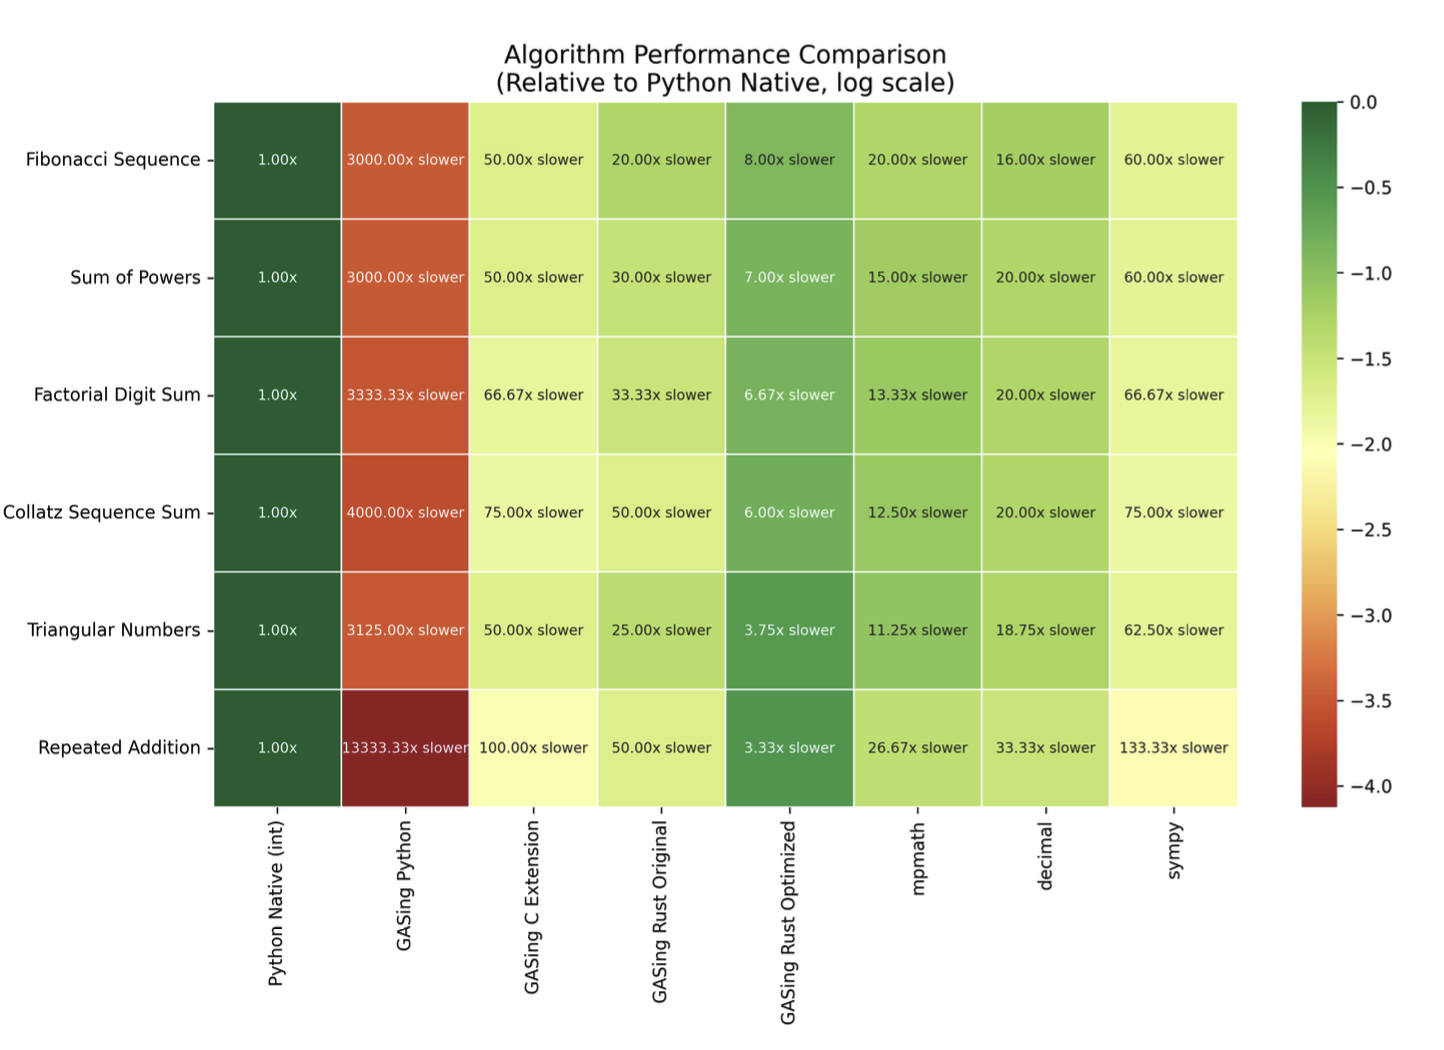
\includegraphics[width=\linewidth]{images/AlgorithmPerformanceComparison.png}
  \caption{Algorithmic Arithmetic}
  \label{fig:algorithmperformancecomparison}
\end{figure}



Looking ahead, these performance tests will be extended to arithmetic calculations that directly underpin large language model (LLM) inferencing. Since all inference operations in LLMs are ultimately arithmetic in nature—encompassing matrix multiplications, activations, and token transformations—any improvement in arithmetic efficiency translates directly to faster inference times and lower energy consumption at scale. This means that the resource savings demonstrated in these benchmarks could become highly visible and impactful in real-world AI deployments, especially as LLMs are deployed on increasingly resource-constrained or energy-sensitive platforms.

In summary, optimizing arithmetic operations through GASing principles has the potential to accelerate LLM inference, reduce operational costs, and make advanced AI systems more accessible and sustainable across a wide range of applications.


\section{Computational Advantages}
The GASing method offers several computational advantages that parallel key innovations in modern neural architectures, particularly those found in the Transformer model:
\paragraph{Locality of Reference and Token-Based Processing}

GASing's digit-wise processing conceptualizes numbers as sequences of tokens, similar to how Transformers process words or subwords. Just as the Transformer treats each token in a sentence as a discrete unit to be processed in parallel, GASing treats each digit as a computational token that can be addressed independently:

\begin{itemize}
\item \textbf{Tokenized Numerical Representation}: By treating a number as a sequence of digits, GASing effectively "tokenizes" numerical data. This mirrors how Transformers tokenize language, allowing arithmetic operations to be reframed as operations on token sequences rather than atomic values.
\end{itemize}

\begin{itemize}
\item \textbf{Cache-Friendly Operations}: The lookup-table approach enables high cache locality by organizing digit-wise operations into predictable memory access patterns. Similar to how Transformer's attention mechanism pre-computes key-value pairs, GASing pre-computes digit-wise results, reducing memory latency and improving throughput.
\end{itemize}

\begin{itemize}
\item \textbf{Compression at Representational Level}: This digit-wise representation provides a fundamental form of information compression. By recognizing patterns at the digit level (e.g., repeated digits, special sequences), GASing can compress computational workloads similar to how attention mechanisms compress sequence information through weighted summation.
\end{itemize}
\paragraph{Attention-Like Direct Accessibility and Predictable Branching}

GASing's systematic approach to arithmetic offers attention-like properties when processing multi-digit numbers:

\begin{itemize}
\item \textbf{Direct Digit Access}: Similar to how self-attention allows any position in a sequence to directly interact with any other position (O(1) path length), GASing's digit-wise processing enables direct access to any digit regardless of its position. This is especially powerful for operations that benefit from examining digits in specific positions.
\end{itemize}

\begin{itemize}
\item \textbf{Rule-Based Position Attention}: The systematic rule-based approach creates a form of "positional attention" where computational patterns are determined by digit positions and their relationships, much like how positional encodings in Transformers help the model understand sequence order.
\end{itemize}

\begin{itemize}
\item \textbf{Reduced Branch Mispredictions}: Like the deterministic attention mechanism in Transformers that avoids recurrent branching, GASing's predictable operation sequences reduce branch mispredictions in processor pipelines. This is particularly valuable in cases where traditional algorithms would have data-dependent branches.
\end{itemize}
\paragraph{Parallelization and Distributed Processing}

The digit-wise nature of GASing creates natural parallelization opportunities that mirror the Transformer's parallel processing capabilities:

\begin{itemize}
\item \textbf{Position-wise Processing}: Just as the Transformer applies the same feed-forward network to each position independently, GASing applies identical digit-wise operations across positions. This enables SIMD (Single Instruction, Multiple Data) optimization at the hardware level.
\end{itemize}

\begin{itemize}
\item \textbf{Granular Task Distribution}: GASing naturally decomposes arithmetic into smaller, independent sub-tasks that can be distributed across processing units, similar to how Transformer's multi-head attention parallelizes attention computations across multiple representation subspaces.
\end{itemize}

\begin{itemize}
\item \textbf{Constant Path Length Operations}: Like the Transformer's attention mechanism that maintains a constant computational path length regardless of sequence length, GASing's pattern-based approach provides constant-time operations for certain patterns regardless of digit count.
\end{itemize}
\paragraph{Information Compression and Pattern Recognition}

GASing represents a fundamental form of information compression that begins at the representational level:

\begin{itemize}
\item \textbf{Pattern-Specific Optimizations}: By identifying and exploiting digit patterns (repeating digits, special sequences), GASing achieves a form of numerical "semantic compression" analogous to how attention mechanisms learn to focus on relevant tokens while ignoring irrelevant ones.
\end{itemize}

\begin{itemize}
\item \textbf{Compositional Understanding}: GASing parses numbers as compositional entities with internal structure, much like how Transformers understand sentences as structured sequences. This allows arithmetic operations to leverage the compositional nature of numerical representation itself.
\end{itemize}

\begin{itemize}
\item \textbf{Adaptive Processing Depth}: For simple patterns, GASing can use shallow processing (direct lookup); for complex patterns, it can apply deeper, recursive processing—parallel to how Transformer layers process simple and complex linguistic patterns with varying attention distributions.
\end{itemize}


\section{Pedagogical Applications}
The GASing arithmetic method offers profound pedagogical advantages by making explicit the deep connections between elementary arithmetic and advanced mathematical concepts. By systematically reducing all operations to variations of addition while maintaining a digit-wise perspective, GASing provides students with a concrete pathway to understanding abstract algebraic structures and theoretical computer science principles.
\paragraph{Foundational Concepts Through Digit-Wise Operations}


\noindent\textbf{\textbf{Recursive Extensibility of Place Value}:} GASing's segment-wise processing demonstrates how the place value system is recursively extensible. Each digit position functions as a self-similar computational unit, mirroring the structure of formal languages and automata theory. This perspective helps students see arithmetic as a formal system with well-defined transformation rules.



\noindent\textbf{\textbf{From Concrete to Abstract Reasoning}:} The progression from single-digit addition to multi-digit operations and beyond illustrates how complex systems emerge from simple, well-defined rules—a fundamental concept in theoretical computer science. Students learn to recognize how higher-level abstractions are built from primitive operations.

\paragraph{Algebraic Structures in Elementary Arithmetic}

GASing's approach naturally leads students to discover abstract algebraic concepts through concrete numerical examples:


\noindent\textbf{\textbf{Monoidal Structure of Addition}:} The method's foundation on addition directly demonstrates the monoidal structure $(\mathbb{N}, +, 0)$, where:


\noindent The set of natural numbers is closed under addition


\noindent Addition is associative (crucial for parallel processing)


\noindent Zero serves as the identity element



\noindent\textbf{\textbf{Group-Theoretic Patterns}:} Through complement-based subtraction, students encounter their first examples of inverse operations, laying the groundwork for understanding group theory. The digit-wise approach makes these abstract concepts tangible by grounding them in familiar numerical operations.

\paragraph{Computational Thinking and Pattern Recognition}


\noindent\textbf{\textbf{Algorithmic Decomposition}:} GASing's step-by-step methodology teaches students to break down complex operations into simpler, manageable components—a core principle of computational thinking.



\noindent\textbf{\textbf{Pattern Recognition and Optimization}:} By working with digit patterns, students develop skills in identifying computational shortcuts and optimizations, directly applicable to algorithm design and analysis.



\noindent\textbf{\textbf{Finite State Automata}:} The carry propagation mechanism in multi-digit addition serves as an accessible introduction to finite state machines, with each digit position representing a state transition based on the current digit and incoming carry.

\paragraph{Pedagogical Advantages for Advanced Topics}


\noindent\textbf{\textbf{Topological Properties of Computation}:} The segment-wise processing in GASing illustrates how computational complexity can be managed through appropriate problem decomposition—a concept that scales to advanced topics in computational topology and distributed systems.



\noindent\textbf{\textbf{Category Theory Connections}:} The method's emphasis on compositionality and universal properties provides an intuitive entry point to category theory concepts, where addition serves as a prototypical example of a monoidal operation.



\noindent\textbf{\textbf{Type Systems and Formal Verification}:} GASing's explicit treatment of digit constraints and carry propagation introduces students to concepts of type safety and formal verification in a concrete, numerical context.

\paragraph{Cognitive Benefits and Practical Applications}


\noindent\textbf{\textbf{Reduced Cognitive Load}:} By focusing on a single core operation (addition) and systematically building complexity, GASing aligns with cognitive load theory, making advanced mathematical concepts more accessible.



\noindent\textbf{\textbf{Transferable Problem-Solving Skills}:} The pattern recognition and decomposition strategies learned through GASing transfer to programming, algorithm design, and other STEM disciplines.



\noindent\textbf{\textbf{Bridging Symbolic and Numerical Reasoning}:} The method's emphasis on the structural aspects of arithmetic helps students develop the ability to move fluidly between concrete computation and abstract reasoning.


Educational observations demonstrate that students who learn arithmetic through the GASing method develop not just computational fluency, but also a deeper appreciation for the underlying mathematical structures. This foundation enables them to approach advanced topics in computer science and mathematics with confidence, seeing the connections between elementary operations and complex theoretical constructs. The method's emphasis on a minimal, coherent operational vocabulary—grounded in addition but extending to higher mathematics—provides a powerful framework for developing both technical skills and conceptual understanding across the mathematical sciences.


\section{Future Directions and Discussion}
As artificial intelligence advances, the challenge of verifying and interpreting complex reasoning grows ever more critical. The Absolute Zero Reasoner (AZR) paradigm demonstrates that it is possible to achieve state-of-the-art reasoning capabilities without any human-curated data, relying solely on self-play and verifiable arithmetic operations as the grouding truth. This paradigm shift aligns directly with the GASing philosophy: arithmetic, especially addition and its extensions, provides a self-sufficient, axiomatically grounded framework for verifying the correctness of reasoning—independent of external supervision, hardware architecture, or computational paradigm.
\paragraph{The GASing Method as a Universal Computational Framework}

\textbf{By grounding AI-powered reasoning in well-documented, human-understandable conceptual abstractions like addition, we establish a truly universal computational framework with several critical properties:}

\begin{itemize}
\item \textbf{Platform-Agnostic:} The GASing framework remains equally valid and effective across all computing platforms:
\end{itemize}
  - Classical von Neumann architectures
  - Neuromorphic processors
  - Quantum computing systems (gate-based, annealing-based, or photonic)
  - Future computational paradigms not yet conceived

\begin{itemize}
\item \textbf{Algorithm-Agnostic:} Verification mechanisms depend solely on the mathematical properties of addition, not on specific algorithmic implementations:
\end{itemize}
  - Independent of programming language or software framework
  - Transcends differences between symbolic and neural approaches
  - Applicable to both deterministic and probabilistic methods
  - Maintains validity across domain-specific optimization techniques

\begin{itemize}
\item \textbf{Resource-Agnostic:} The framework provides a universal unit of resource measurement applicable across computational contexts:
\end{itemize}
  - Independent of specific hardware constraints (memory, processing units, energy)
  - Scalable from edge devices to supercomputers
  - Adaptable to varying precision requirements
  - Enables precise resource accounting in heterogeneous computing environments

\begin{itemize}
\item \textbf{Axiomatically Grounded:} Arithmetic serves as a definitive framework that establishes clear boundaries of rational precision:
\end{itemize}
  - Provides a formal basis for all computational correctness claims
  - Establishes unambiguous termination conditions for decision processes
  - Enables verification chains with guaranteed consistency
  - Creates a universal standard for precision and approximation

The correctness verification mechanisms can always be traced back to the axiomatic definition of addition and the finite vocabulary admitted in each application context. While this vocabulary adapts to different domains, it remains terminable in decision processes because it builds on fundamental arithmetic operations with clear termination conditions, regardless of the physical substrate performing the calculation.
\paragraph{Arithmetic as the Universal Computational Substrate}

It is crucial to recognize that all computations—regardless of their apparent complexity or implementation—reduce to arithmetic operations at their logical foundation:

\begin{itemize}
\item \textbf{Universal Computational Mapping:}
\end{itemize}
  - Every token prediction in language models → Matrix operations → Addition sequences
  - Quantum gate operations → Unitary transformations → Complex number arithmetic
  - Neural network activations → Weighted sums and non-linear functions → Addition and multiplication
  - Symbolic reasoning → Logical operations → Arithmetic on truth values

\begin{itemize}
\item \textbf{Hardware-Independent Optimization:}
\end{itemize}
  - Pre-computation of recurring patterns yields benefits regardless of physical implementation
  - Pattern recognition strategies remain valid across all computing architectures
  - Resource optimization techniques are transferable between computational paradigms
  - Lookup mechanisms provide acceleration whether implemented in classical or quantum systems

Similar to the arguments presented in AZR's framework for abduction, deduction, and induction is not merely a high-level abstraction; each of these reasoning modes is ultimately reducible to arithmetic operations, most notably matrix dot products. These operations serve as the computational substrate for verifying hypotheses, generating explanations, and drawing inferences. By grounding all reasoning in arithmetic, GASing together offer a path toward:

1. \textbf{Self-Sufficient Verification of Truth}: Arithmetic rules, being universally accepted and axiomatically defined, enable models to autonomously verify the correctness of their outputs. This eliminates the need for human-provided labels or curated datasets, allowing for open-ended, scalable learning and reasoning.

2. \textbf{Unified Framework for Reasoning}: Abduction (hypothesis generation), deduction (logical consequence), and induction (pattern discovery) can all be formalized as arithmetic operations—often as matrix multiplications or dot products—within the AZR paradigm. This unification simplifies the architecture of reasoning systems and ensures that all forms of inference are ultimately transparent and verifiable.

3. \textbf{Enhanced AI Interpretability and Trust}: By reducing complex reasoning to sequences of arithmetic steps, the entire process becomes auditable and explainable. Each step can be traced back to fundamental operations, making it possible to verify not just the final answer but the entire chain of reasoning.

4. \textbf{Bridging Symbolic and Sub-symbolic AI}: The arithmetic foundation enables seamless integration between symbolic logic (rules, proofs) and sub-symbolic computation (matrix operations, neural activations). This hybrid approach supports both human-understandable explanations and efficient machine computation.

5. \textbf{Preparation for Autonomous, Superhuman AI}: As demonstrated by AZR, models can propose, solve, and verify tasks entirely through self-play, guided by arithmetic truth. This prepares AI systems for a future where they must operate and improve independently, without relying on human supervision or external data.

As detailed in recent work on the Absolute Zero Reasoner (AZR), the three primary modes of learning—deduction, abduction, and induction—can be mapped directly onto the fundamental arithmetic operations of subtraction, addition, and multiplication/division, respectively. Deduction resembles subtraction, isolating unknowns from knowns; abduction parallels addition, combining elements to reach a target; and induction aligns with multiplication/division, generalizing or partitioning patterns. This mapping is not merely metaphorical: AZR operationalizes each reasoning mode as arithmetic, typically via matrix dot products and related operations. Thus, the logical and functional structure of arithmetic is sufficiently expressive to serve as the substrate for all forms of inference, unifying symbolic and sub-symbolic reasoning.

Anthropic's groundbreaking work on monosemanticity ("Towards Monosemanticity: Decomposing Language Models With Dictionary Learning") provides compelling evidence for this approach. Their research demonstrated that sparse autoencoders can decompose complex language models into thousands of interpretable features, with each feature representing a specific, meaningful pattern—similar to how GASing decomposes complex arithmetic into modular, pattern-recognizing steps. They discovered that just 512 neurons can effectively represent tens of thousands of features, and these features connect in "finite-state automata"-like systems to implement complex behaviors.

This directly parallels GASing's principle of pattern decomposition: where Anthropic finds that complex language behaviors can be decomposed into interpretable components, GASing shows that complex arithmetic can be decomposed into pattern-driven addition operations. Both approaches tackle the "curse of dimensionality" by identifying compositional building blocks that make complex systems interpretable and controllable.

Furthermore, Anthropic demonstrated that these monosemantic features can be used to intervene on and steer transformer generation—activating a specific feature (like "base64" or "Arabic script") causes the model to generate text with those characteristics. In the GASing framework, recognizing specific numerical patterns similarly allows for targeted optimizations and controlled behaviors.

The key insight connecting these approaches is that dictionaries and lookup tables are essentially pre-computed results—cached knowledge that can dramatically accelerate reasoning when leveraged appropriately. This parallel between GASing and Anthropic's approach reveals a profound connection between mental arithmetic and neural computation.
\paragraph{Monosemanticity and Digit-Wise Decomposition}

Anthropic's dictionary learning approach in their Monosemantic research represents a breakthrough in neural network interpretability through decomposition. Their technique addresses the "polysemanticity problem" where individual neurons encode multiple concepts simultaneously, making interpretation difficult. Using sparse autoencoders, they decompose these mixed neural activations into thousands of interpretable "features" or "basis vectors" that represent singular concepts—such as specific text patterns, data formats, or linguistic structures.

This decomposition is structurally analogous to how GASing decomposes complex arithmetic operations into digit-wise patterns:

- \textbf{GASing's Lookup Tables}: Break down arithmetic operations into pre-computed digit-wise patterns stored in mental lookup tables
- \textbf{Anthropic's Dictionary Elements}: Break down neural activations into interpretable monosemantic features stored in sparse feature vectors

In both cases, complex operations (whether arithmetic calculations or neural processes) are transformed into combinations of simpler, more interpretable components that can be efficiently accessed and combined.
\paragraph{From Polynomial Types to Computational Efficiency}

This dictionary-based filtering methodology bears remarkable structural similarity to \textbf{[[Polynomial Functors]]} as in [[Category Theory]], where arithmetic rules denote different types of information and their compositional relationships. Just as Polynomial Functors use addition to represent alternatives and multiplication to represent combinations, both GASing's lookup patterns and Anthropic's dictionary features create formal algebras for organizing computational resources:

- In GASing: Digit patterns become the "vocabulary" of arithmetic, with rules for composition that minimize cognitive effort
- In Anthropic's approach: Dictionary features become the "vocabulary" of neural computation, with sparse activations that minimize computational resources

The dictionary learning approach is fundamentally a form of resource-aware computation that aligns directly with [[Linear Logic]] principles—each feature is consumed exactly once in reconstructing the neural activation, just as each digit pattern is consumed exactly once in GASing's mental calculations.
\paragraph{Practical Implications for Computation}

The digit-wise pattern extraction strategy in GASing arithmetic represents a fundamental breakthrough in computational efficiency, with deep connections to advanced mathematical frameworks like [[Homological Algebra]] and [[Topological Data Analysis]] (TDA). These fields, at the forefront of modern data science, employ similar pattern recognition and dimensional reduction techniques to extract meaningful structure from complex datasets.

The algebraic topology underpinning these approaches—particularly the computation of persistent homology in TDA—shares striking parallels with GASing's digit-wise operations. Both frameworks excel at identifying and exploiting qualitative features that persist across multiple scales, enabling more efficient representation and manipulation of complex data structures. This connection to [[Persistent Homology]] and [[Morse Theory]] provides a rigorous mathematical foundation for understanding how GASing's pattern-based approach achieves its remarkable computational efficiency.

Just as GASing enables humans to perform complex mental calculations through pattern recognition and recombination, modern neural architectures leverage similar principles rooted in [[Sheaf Theory]] and [[Category Theory]]. In Anthropic's experiments with Claude 3 Sonnet, the decomposition of neural layers into interpretable features mirrors the way [[Čech Complexes]] in TDA capture topological features across different scales. This multi-scale pattern recognition allows systems to:

1. \textbf{Dynamically renormalize} computational processes using techniques inspired by [[Renormalization Groups]] in theoretical physics
2. \textbf{Cache and reuse} intermediate results through structures analogous to [[Cohomology Operations]] in algebraic topology
3. \textbf{Adaptively allocate resources} using methods that parallel [[Barcodes]] in persistent homology, which track the persistence of topological features across scales

The mathematical framework of [[Spectral Sequences]] from homological algebra provides a powerful lens for understanding how GASing's digit-wise operations can efficiently navigate complex computational landscapes. This connection to advanced algebraic topology explains why GASing's approach remains effective even as computational paradigms evolve—the underlying mathematical structures are fundamentally stable across different representations and implementations.

The real challenge, for both humans and machines, is to access these pre-computed patterns with minimal resource expenditure while adapting retrieval strategies to the local context. The GASing framework's modular, segment-wise approach provides a principled foundation for this adaptive resource management, with deep connections to [[Sheaf Cohomology]] and its applications in distributed systems and data analysis.

By establishing addition as the foundational operator for all reasoning mechanisms, GASing provides an abstract, universal unit of resource measurement that finds elegant expression in the language of [[Category Theory]] and [[Homotopy Type Theory]]. This approach enables precise assessment of computational requirements through the lens of [[Euler's Characteristic]] and other topological invariants, creating a rigorous framework for reasoning about computational complexity across different scales and representations.

\textbf{The profound advantage of this approach is that it provides a mathematical foundation for understanding how complex computations can be decomposed into simpler, more manageable components—a principle that lies at the heart of both GASing arithmetic and modern topological methods in data science.} This separation creates an enduring bridge between theoretical verification and practical optimization across all computational paradigms. Even as we transition through classical computing to neuromorphic systems and ultimately to mature quantum computing, the core verification mechanisms remain mathematically identical because they depend only on the abstract properties of addition and topological invariants, not on the physical substrate performing the operations.

More importantly, this mathematical framing enables us to view each LLM as a custom numerical system with its own unique arithmetic properties, where the token distributions, weight matrices, and activation patterns constitute a rich numerical ecosystem. The principles of [[Representation Stability]] from [[homological algebra]] suggest that many of the patterns we discover in these systems will remain stable even as the underlying models scale, providing a powerful tool for model compression and optimization. By identifying and exploiting these stable patterns—much like how TDA identifies persistent topological features—we can achieve significant computational savings while preserving model accuracy and interpretability.

These insights are not merely theoretical: they provide immediately actionable approaches for optimizing existing AI systems while pointing the way toward more efficient and interpretable architectures. The deep mathematical connections between GASing arithmetic, homological algebra, and topological data analysis suggest that we are only beginning to understand the full potential of these approaches for building the next generation of intelligent systems.


\section{Conclusion}
\paragraph{Cultural and Historical Context: Ethno Arithmetic and Fractal Patterns}

The GASing method finds profound resonance with the work of Professor Ron Eglash on \textbf{Ethno Arithmetic} and fractal patterns in Indigenous knowledge systems. Eglash's research (Eglash, 1999) demonstrates how many African, Native American, and other Indigenous cultures developed sophisticated mathematical concepts through fractal patterns in their art, architecture, and social organizations. These patterns, often embedded in cultural practices, represent an early form of \textbf{progressive function application} and \textbf{self-similar computation} that predates Western formal mathematics.

GASing's digit-wise, cell-like modules parallel the recursive, self-similar structures found in Indigenous fractal designs, where complex patterns emerge from the repeated application of simple rules—a principle that mirrors GASing's approach to arithmetic through the progressive application of addition. The \textbf{combinatorial patterns} in GASing's digit-wise processing echo the recursive geometric transformations observed in African fractals, where simple scaling rules generate complex, computationally rich structures.

This connection is particularly significant because it suggests that GASing's approach is not merely a technical innovation but part of a broader human tradition of pattern-based computation. By recognizing these parallels, GASing bridges modern computational thinking with historical mathematical practices, creating a more inclusive framework that honors diverse mathematical traditions while providing a foundation for future computational paradigms.
\paragraph{Computational Foundations}

The GASing arithmetic method positions the foundational architecture of computing tasks by elevating addition to the role of meta-operator—a universal primitive from which all arithmetic logic operations can be systematically constructed, analyzed, and verified. This reductionist approach is not merely a theoretical exercise; it provides a practical, measurable framework for assessing resource consumption, numerical precision, and logical correctness in both human and machine reasoning. As modern LLM technologies have conclusively demonstrated, even \textbf{the most sophisticated reasoning and content generation processes}—from poetry composition to mathematical proof generation—\textbf{can be carried out with arithmetic operations} as their fundamental computational substrate. The seemingly magical capabilities of these systems emerge entirely from operations that, at their core, are nothing more than carefully orchestrated \textbf{patterns of addition and multiplication}.

By \textbf{conceptually decomposing} complex operations such as multiplication, subtraction, and division into sequences of segment-wise additions, GASing enables explicit quantification of computational effort: every operation is traceable to a countable set of addition-equivalent steps. This transparency allows for rigorous evaluation and optimization of both cognitive and computational resource usage, offering a clear metric for comparing algorithms, implementations, or even reasoning strategies. Such granularity is invaluable for designing systems—human or artificial—that must operate within strict resource constraints, whether those are working memory, processing time, or energy consumption.

GASing’s focus on addition as the core operator also underpins a unified, cross-referential decision framework. By expressing all arithmetic logic in terms of addition, the method ensures that every step is both interpretable and verifiable, supporting robust provenance tracking and error detection. This unification bridges symbolic and sub-symbolic computation, aligning the clarity of rule-based logic with the efficiency of neural and matrix-based operations. The result is a system where numerical precision and logical correctness are not competing priorities, but mutually reinforcing outcomes of a single, transparent process.

Originally conceived to accelerate arithmetic calculation and reduce cognitive load for learners, GASing’s segment-wise, pattern-driven approach is grounded in well-established cognitive principles, such as chunking and resource preservation. It empowers users to adapt the granularity of operations to their own cognitive limits, minimizing mental effort while maximizing accuracy and speed. This adaptability is mirrored in modern AI, where resource management and interpretability are critical for scaling intelligent systems.

In summary, GASing arithmetic is more than a pedagogical innovation—it is a rigorous, interpretable, and scalable substrate for reasoning that bridges the gap between human cognition and machine computation. By grounding all operations in addition, GASing delivers a framework where every logical step is measurable, every result is verifiable, and every computation is optimized for resource efficiency.

At a deeper level, GASing establishes \textbf{\textbf{\textit{addition}}} as a universal atomic "token" of computational effort—a fundamental unit of measure that enables precise resource accounting across all computational contexts, from silicon chips to human minds. This resource-aware arithmetic framework redefines how we attribute and measure cognitive and computational work, creating a unified currency of effort that makes the cost of any reasoning process explicitly quantifiable. Each "adding action" becomes a credit unit within a universal ledger of computational activity, allowing systems to track, allocate, and optimize resources with unprecedented granularity. This approach transcends traditional hardware-specific metrics (like CPU cycles or memory usage) to establish a hardware-agnostic measure of fundamental reasoning operations.

This philosophical reinterpretation of what counting fundamentally means represents a major advancement in how we conceptualize and accumulate knowledge about the world. By establishing the addition operation as the atomic unit of reasoning, GASing provides a common denominator for measuring all forms of information processing, creating a bridge between disparate computational paradigms—quantum, neural, symbolic—and human cognition. It enables precise verification chains that can track not just the results of computation, but the exact resource cost of arriving at those results, providing a meta-level framework for reasoning about reasoning itself.

Intellectually, grounding all computational tasks in a single unifying operator yields an additional, profound benefit: it encourages both human and machine minds to converge on a shared pattern of reasoning. This shared pattern not only accumulates experience and impressions, but also aligns prior intentions and fosters deeper mutual understanding. In the abstract, aligning minds—whether individual, collective, or artificial—around a common operator is a necessary condition for establishing a unified theory of learning. Only by sharing such a foundational operator can human, machine, or organizational learning truly converge on a common framework, enabling the transfer and accumulation of knowledge, experience, and intention across all forms of intelligence.

As AI systems become increasingly autonomous and integrated into human workflows, such foundational clarity and measurability will be essential for ensuring trust, transparency, and continual improvement in both artificial and human intelligence. Modern LLMs have definitively proven that even the most advanced cognitive-seeming tasks—from multimodal reasoning to creative problem-solving—ultimately resolve to sequences of arithmetic operations. This revelation means that optimizing these fundamental operations is not merely an engineering detail but a strategic imperative with cascading benefits for AI capabilities, energy consumption, and accessibility. By \textbf{minimizing the resource footprint of these basic arithmetic operations through the principles outlined in GASing}, we can achieve dramatic improvements in these proven useful and pragmatic AI applications regardless of their apparent complexity or sophistication.

\textbf{Crucially, by grounding AI-powered reasoning in well-documented and human-understandable conceptual abstractions, GASing eliminates dependencies on specific hardware or software implementations.} The correctness verification process can always be traced back to the axiomatic definition of addition and the finite vocabulary admitted in each application context. This creates an adaptive yet fundamentally terminable reasoning framework—one that can evolve with technological advances without losing its verifiability. As hardware implementations evolve from classical computing to neuromorphic processors or quantum computers, the GASing verification mechanisms remain stable and interpretable to humans because they depend on mathematical properties, not implementation details. This ensures a consistent standard of correctness while enabling continuous innovation in the underlying technologies.

GASing's commitment to a minimal, interpretable operational vocabulary thus stands as both a practical solution and a philosophical imperative for the future of collaborative reasoning—one where the economics of knowledge acquisition can be precisely quantified, compared, and optimized across the full spectrum of computational agents, from the simplest calculator to the most sophisticated AI system to the human mind itself.

% Appendix section
\appendix
% Appendix
% This appendix contains supplementary material, proofs, extended algorithms, and additional data relevant to the GASing Arithmetic System.

\section{Appendix I: GASing Addition Algorithm}
\label{appendix:addition}
\begin{lstlisting}[language=Python,caption={GASing Addition Algorithm}]
function GASing_Addition(a, b):
    result = ""
    carry = 0
    
    # Pad the shorter number with leading zeros
    a = pad_with_zeros(a, len(b))
    b = pad_with_zeros(b, len(a))
    
    # Process from left to right
    for i in range(0, len(a)):
        # Add digits and carry
        digit_sum = int(a[i]) + int(b[i]) + carry
        
        # Determine new digit and carry
        if digit_sum > 9:
            carry = 1
            digit = digit_sum - 10
        else:
            carry = 0
            digit = digit_sum
        
        result += str(digit)
    
    # Add final carry if necessary
    if carry > 0:
        result += str(carry)
        
    return result
\end{lstlisting}

\section{Appendix II: GASing Multiplication Algorithm}
\label{appendix:multiplication}
\begin{lstlisting}[language=Python,caption={GASing Multiplication Algorithm (Conceptual)}]
function GASing_Multiplication(a, b):
    # Initialize a grid to store partial products (results of single-digit multiplications)
    # The dimensions of the grid depend on the number of digits/segments in a and b.
    # For example, if a has M segments and b has N segments, grid is N x M.
        
    grid = initialize_partial_product_grid(a, b) # Each grid[i][j] = segment_b[i] * segment_a[j]
        
    # The core of multiplication is now to sum the values in this grid in a structured way.
    # This can be visualized as summing diagonals or columns, applying GASing addition.
    # For simplicity, imagine a function that collects these partial products and sums them
    # using the previously defined GASing_Addition logic, managing carries appropriately.

    final_product = "0"
    # Iterate through the grid, treating each row (or shifted row) as a number to be added.
    # This is a conceptual representation; actual implementation involves careful alignment and summation.
    for i in range(len(b)):
        partial_sum_for_row_i = "0"
        for j in range(len(a)):
            # Conceptually, each grid[i][j] contributes to a sum that is then added.
            # A more direct approach involves summing diagonals or columns with carries.
            # This step is a placeholder for the detailed grid summation logic.
            # For instance, grid[i][j] is like (digit_b[i] * digit_a[j]) * 10^(position_factor)
            # These terms are then summed up.
            pass # Detailed grid summation logic would be here.

    # A more accurate representation of grid summation:
    # 1. Calculate all single-segment products: product_ij = segment_a[j] * segment_b[i]
    # 2. Arrange these products in a grid, aligning them according to their place value.
    # 3. Sum the columns of this grid using GASing_Addition, propagating carries.

    # Example (conceptual): Summing diagonals of the grid of partial products
    # result = sum_grid_diagonals_with_gasing_addition(grid)

    # Simplified placeholder for the complex summation logic:
    # Assume 'grid_to_result' performs the systematic addition of partial products
    # according to GASing principles (left-to-right, carry management).
    
    result = perform_structured_addition_on_grid(grid, GASing_Addition_function_pointer)

return result
\end{lstlisting}

\section{Appendix III: GASing Subtraction and Division Algorithms}
\label{appendix:subtraction}
\begin{lstlisting}[language=Python,caption={GASing Subtraction Algorithm}]
function GASing_Subtraction(a, b, base=10):
    # Ensure a and b are of the same length for complement calculation
    # This might involve padding the shorter number or defining a fixed width.
    # For simplicity, assume a and b are positive integers represented as strings.
    num_digits = max(len(a), len(b))

    a_padded = pad_with_zeros(a, num_digits)
    b_padded = pad_with_zeros(b, num_digits)

    # Calculate n's complement of b (e.g., ten's complement for base 10)
    # This involves (base^num_digits - b_padded)
    # A common method: ( (base-1)'s_complement of b_padded ) + 1
    b_complement_n_minus_1 = ""
    for digit_char in b_padded:
        b_complement_n_minus_1 += str((base - 1) - int(digit_char))

    # Add 1 to get n's complement (e.g., ten's complement)
    # This addition itself can use a simplified version of GASing_Addition or direct logic
    one_str = pad_with_zeros("1", num_digits)
    b_complement_n = GASing_Addition(b_complement_n_minus_1, one_str) # Assuming base compatibility
    # Handle potential overflow from complement addition if b_complement_n exceeds num_digits
    if len(b_complement_n) > num_digits and b_complement_n.startswith('1'): # Check for leading '1' from carry
        b_complement_n = b_complement_n[1:] # Keep only num_digits
    else:
        b_complement_n = pad_with_zeros(b_complement_n, num_digits)

    # Perform a + (n's complement of b)
    # The GASing_Addition function is used here.
    sum_with_complement = GASing_Addition(a_padded, b_complement_n) # Ensure base compatibility

    # Interpret the result
    if len(sum_with_complement) > num_digits and sum_with_complement.startswith('1'): # Overflow carry indicates positive result
        result = sum_with_complement[1:] # Discard overflow carry
        is_negative = False
    else:
        # No overflow carry indicates negative result or zero
        # The result is negative, and its magnitude is the n's complement of sum_with_complement
        # For simplicity, we'll just flag it as negative and take complement again for magnitude
        # (or handle based on specific complement arithmetic rules)
        if sum_with_complement == pad_with_zeros("0", num_digits):
            result = sum_with_complement
            is_negative = False
        else:
            # Recalculate n's complement of sum_with_complement to get magnitude
            temp_complement_n_minus_1 = ""
            sum_with_complement_padded = pad_with_zeros(sum_with_complement, num_digits)
            for digit_char in sum_with_complement_padded:
                temp_complement_n_minus_1 += str((base - 1) - int(digit_char))
            result = GASing_Addition(temp_complement_n_minus_1, one_str) # Magnitude
            if len(result) > num_digits and result.startswith('1'):
                result = result[1:]
            else:
                result = pad_with_zeros(result, num_digits)
            is_negative = True
            
    return result, is_negative
\end{lstlisting}

\begin{lstlisting}[language=Python,caption={GASing Division Algorithm}]
function GASing_Division(dividend, divisor, base=10):
    if divisor == pad_with_zeros("0", len(divisor)):
        return "Error: Division by zero"
    quotient = "0"
    current_dividend = dividend
    one = pad_with_zeros("1", len(quotient)) # For incrementing quotient

    # Repeatedly subtract divisor from current_dividend
    # We need a comparison function: is_greater_or_equal(num1, num2)
    while is_greater_or_equal(current_dividend, divisor):
        subtraction_result, is_neg = GASing_Subtraction(current_dividend, divisor, base)
        if is_neg: # Should not happen if is_greater_or_equal is correct
            break 
        current_dividend = subtraction_result
        quotient = GASing_Addition(quotient, one) # Increment quotient
        # Ensure 'one' is padded correctly if quotient grows
        if len(quotient) > len(one):
            one = pad_with_zeros("1", len(quotient))
        elif len(one) > len(quotient):
            quotient = pad_with_zeros(quotient, len(one))

    remainder = current_dividend
    return quotient, remainder
\end{lstlisting}



% Acknowledgments
\section*{Acknowledgments}
The authors would like to thank the AI Toba Project and IT Del for their support.

% Bibliography
\section*{References}
\nocite{*}
\bibliographystyle{IEEEtran}
\bibliography{bibliography}

% End of document
\begin{abstract}
                                     \documentclass[11pt,a4paper]{article}
\usepackage[utf8]{inputenc}
\usepackage[T1]{fontenc}
\usepackage{graphicx}
\usepackage{amsmath}
\usepackage{amssymb}
\usepackage{listings}
\usepackage{xcolor}
\usepackage{hyperref}
\usepackage{float}
\usepackage{booktabs}
\usepackage{geometry}
\usepackage{parskip}
\usepackage{enumitem}
\usepackage{titlesec}
\usepackage{setspace}
\onehalfspacing
\geometry{margin=1in}
\titleformat{\section}{\Large\bfseries}{\thesection}{1em}{}
\titleformat{\subsection}{\large\bfseries}{\thesubsection}{1em}{}
\titleformat{\subsubsection}{\bfseries}{\thesubsubsection}{1em}{}
\lstset{
    basicstyle=\ttfamily\small,
    breaklines=true,
    frame=single,
    numbers=left,
    numberstyle=\tiny,
    numbersep=5pt,
    showstringspaces=false,
    keywordstyle=\color{blue},
    stringstyle=\color{red},
    commentstyle=\color{green!60!black},
    morekeywords={function,return,if,else,for,while,import,as,from,class,def,True,False,None}
}
\hypersetup{
    colorlinks=true,
    linkcolor=blue,
    filecolor=magenta,
    urlcolor=cyan,
    pdftitle={GASing Arithmetic Method},
    pdfpagemode=FullScreen,
}
\title{GASing Arithmetic Method: A Novel Approach to Computation}
\author{}
\date{\today}
\begin{document}
\maketitle
\tableofcontents
\newpage
\section{The GASing Arithmetic Method: A Novel Approach to Computation}
\section{The GASing Arithmetic Method: A Novel Approach to Computation}
\emph{May 3, 2025}

\subsection{Abstract}
The [[GASing Arithmetic]] method introduces a foundational paradigm for numerical computation at the intersection of human cognition, cultural mathematics, and artificial intelligence. Drawing inspiration from Eglash's work in [[Ethno Arithmetic]] and fractal patterns in indigenous knowledge systems, GASing demonstrates how culturally-grounded mathematical insights can inform modern computational frameworks. In an era where AI systems increasingly shape and augment human reasoning, there is a critical need for computational approaches that are not only transparent and interpretable but also capable of aligning with fundamental cognitive patterns across diverse cultural contexts. GASing addresses this challenge through the \textbf{progressive application of functions} and \textbf{digit-wise systems as cell-like modules}, establishing \textbf{addition as the universal meta-operator}—the cornerstone of a minimized operational vocabulary from which all arithmetic logic can be systematically constructed, analyzed, and verified. 

This approach leverages the inherent combinatorial patterns in self-similar systems to better compress unnecessary computational efforts. Through digit-wise processing and pattern recognition, GASing enables explicit quantification of computational effort and resource usage, bridging symbolic and neural approaches while supporting robust provenance tracking. The method's cell-like modular architecture, inspired by the fractal patterns found in traditional Indonesian design and other indigenous knowledge systems, allows for efficient information processing by breaking down complex operations into manageable, recombinable units. This unified approach has been successfully implemented in Indonesia's national education program, reaching millions of students and demonstrating how culturally-informed knowledge exchange protocols can be continuously improved at scale. Our findings demonstrate that GASing is not only a mathematically rigorous and pedagogically effective framework, but also a culturally-grounded substrate for interpretable, trustworthy, and resource-efficient AI—laying the groundwork for a unified theory of learning rooted in both universal mathematical principles and diverse cultural expressions of mathematical thinking.

\subsection{1. Introduction}
The rise of large language models and neural computing has fundamentally transformed how humans reason in partnership with machines, yet this transformation brings new challenges in interpretability, verification, and cognitive alignment. \textbf{What is often overlooked is that these sophisticated AI systems—capable of generating human-like text, solving complex reasoning tasks, and exhibiting seemingly advanced cognition—ultimately operate through nothing more than arithmetic operations at their core.} Every transformer attention mechanism, every matrix multiplication, every embedding lookup fundamentally reduces to addition, multiplication, and their derivatives. This reality underscores a profound insight: even the most complex reasoning and generative processes can be carried out with arithmetic operations alone. The GASing method responds to this fundamental truth by reconceptualizing arithmetic operations through a digit-wise, pattern-recognition framework that serves as a universal computational paradigm—\textbf{anchored in the principle of minimizing its operational vocabulary by grounding all arithmetic in the fundamental operator of addition.}

This approach finds deep resonance with the work of Professor Ron Eglash in Ethno Mathematics, which reveals how diverse cultures have developed sophisticated mathematical concepts through everyday practices and artistic expressions. The fractal patterns found in traditional Indonesian batik (see Situngkir and Surya, 2009), African architecture (see Eglash, 1999), and other indigenous knowledge systems demonstrate how complex mathematical thinking emerges naturally across human cultures. GASing builds upon these insights by formalizing how such pattern-based reasoning can inform modern computational frameworks. In Indonesia, this approach has been successfully scaled through national education initiatives, where GASing's principles have been integrated into the mathematics curriculum, reaching millions of students and demonstrating how culturally-grounded mathematical thinking can enhance computational literacy at scale.

By positioning addition as a meta-operator—capable of expressing the meaning of any symbolic token structure—GASing creates a language-agnostic verification framework that is both interpretable and measurable. This reduction to a core operator allows for direct assessment of computational and cognitive resource consumption, transparent verification of reasoning, and systematic arrangement of operations that parallel both transformer attention mechanisms and human chunking strategies. \textbf{Given that modern LLMs execute billions or even trillions of arithmetic operations during inference alone, any optimization of these fundamental operations—through pattern recognition, lookup mechanisms, or structural rearrangement—would yield substantial improvements in efficiency, regardless of the apparent complexity of the higher-level reasoning being performed.} The result is a unified, cross-referential decision framework in which every logical step is both auditable and adaptable to the cognitive limits of users or the architectural constraints of machines.

The name "GASing" derives from Indonesian terms: Gampang (easy), Asyik (enjoyable), and menyenangkan (interesting), reflecting the method’s dual purpose: making arithmetic accessible for human understanding while providing a rigorous foundation for interpretable AI. Originally developed as a pedagogical tool, GASing now stands as a scalable, mathematically rigorous, and philosophically grounded approach—one that not only mirrors key aspects of modern AI architectures, but also fosters the convergence of human, machine, and organizational reasoning on a shared, minimal, and interpretable operational substrate. This commitment to a common operator is both a practical solution and a necessary condition for the emergence of a unified theory of learning and collaborative intelligence.

\subsection{2. Foundational Principles}
The GASing method is built upon several coherent principles designed to demonstrate the transformative power of \textbf{composition and decomposition through digit-wise manipulation of representation systems}. At its essence, GASing provides both a rigorous formalism and an intuitive mental model of resource-awareness, showing how complex arithmetic operations can be systematically constructed from and deconstructed into elemental addition steps. By grounding all arithmetic in compositional patterns of addition, GASing makes resource consumption explicitly visible and quantifiable at every step of the reasoning process. Crucially, this approach establishes a \textbf{resource-aware axiomatic foundation} that derives its power not from statistical patterns or dataset-dependent heuristics, but from the fundamental mathematical properties of addition operations and their compositional nature at the representational level. The resulting framework enables practitioners to perceive, measure, and optimize computational resources with unprecedented clarity—whether those resources are CPU cycles, memory units, or human cognitive capacity. This axiomatic approach to composition ensures that computational correctness and resource efficiency are achieved through principled rules rather than empirical biases, making the system inherently trustworthy across all possible inputs and contexts.

\paragraph{2.1 The Digit-Wise Processing Paradigm}
At its core, GASing employs a digit-wise processing approach that treats numerical segments as \textbf{cell-like modules} within a larger computational organism. This approach doesn't merely break numbers into fixed constituent digits but rather establishes a \textbf{progressive function application} framework where each digit or digit-group functions as an independent computational unit. These units interact through well-defined interfaces (carry/borrow propagations) while maintaining their modular integrity, much like biological cells function within a larger organism.

The boundaries of these arithmetic operations are flexibly defined by utilizing the topological properties of Carry and Borrow propagations between adjacent numerical segments. This creates a \textbf{self-similar computational architecture} where the same fundamental operations apply at multiple scales, from single-digit operations to complex multi-segment calculations. The granularity of these segments can be dynamically determined to optimize arithmetic calculation efficiency, particularly leveraging the observation that operations become highly efficient when all unique combinations of numerical values within these segments can be assessed \emph{a priori}. 

A critical advantage of this approach is its exploitation of \textbf{combinatorial patterns in self-similar systems}. For any given segment size, there exists only a finite set of combinatorial possibilities among pairs of addition operands. These combinations form a \textbf{combinatorial space} that exhibits fractal-like properties—the same patterns of interaction between digits recur at different scales of magnitude. By pre-calculating and storing these patterns in optimized lookup tables, GASing achieves \textbf{computational compression}, dramatically reducing redundant calculations during runtime.

This pre-calculation strategy creates a \textbf{progressive application pipeline} where frequently encountered patterns are processed through highly optimized lookup operations, while less common combinations fall back to more general computational pathways. In contexts like Large Language Model (LLM) inference, where numerical patterns often follow predictable distributions, this approach enables \textbf{adaptive computation}—allocating more resources to common operations while gracefully handling edge cases. The system's ability to tailor its computational approach to both the statistical properties of the input and the available hardware resources (cache sizes, memory hierarchies, etc.) allows for acceleration that scales efficiently with problem complexity.

This refined digit-wise paradigm represents a \textbf{progressive function application} framework that minimizes operational complexity through \textbf{cellular decomposition}. Each digit or digit-group functions as a semi-autonomous computational unit, processing information according to a consistent set of rules while maintaining the flexibility to adapt to different contexts and scales. This approach transforms arithmetic from a monolithic operation into a \textbf{distributed computation} where each cell (digit) contributes to the overall result through local interactions with its immediate neighbors.

By focusing on these \textbf{digit-wise cellular modules}, GASing achieves a form of \textbf{computational compression} where complex operations emerge from the interaction of simpler, well-defined components. This approach aligns with both human cognitive abilities and modern computational architecture through several key principles:

\begin{enumerate}
  \item - \textbf{Human Cognition}: By processing operations at the level of these flexibly defined numerical segments (which can be as small as single digits), GASing leverages established neural pathways for simpler operations (Dehaene, 2011). This modular, segment-based processing keeps the cognitive load for each step manageable, making the system intuitive and easier for human users to verify, even as the definition of a 'segment' adapts for efficiency.
  \item - \textbf{Computational Architecture}: This segment-wise processing, where segments can be optimized for computational efficiency (e.g., to fit register sizes or leverage pre-computed lookup tables for segment-level operations), maps effectively to modern processor capabilities. The ability to dynamically adjust segment sizes and lookup table structures based on the specific computational environment enables optimal utilization of hardware resources, from register sizes and cache hierarchies to SIMD capabilities. Particularly noteworthy is how GASing naturally aligns with [[SIMD Within A Register]] ([[SWAR]]) techniques, which allow multiple small values to be processed simultaneously within a single processor register. By carefully selecting segment sizes to match register subword boundaries, GASing can exploit parallelism at the instruction level without requiring special vector instructions. This approach is highly dependent on the numeric values of the inputs—specific digit patterns can be arranged to avoid carry chains between segments, enabling true parallel processing of multiple additions within a single register. For example, with 64-bit registers, eight 8-bit segments can be processed simultaneously if the operands are properly arranged to prevent inter-segment carry propagation. Reducing operations to their simplest form at the segment level (e.g., segment addition and inter-segment carry/borrow) allows for granular understanding, control of computational resources, and potential for optimized hardware implementations that can adaptively select between scalar, SWAR, or full SIMD execution paths based on the specific digit patterns present in the inputs.
\end{enumerate}

This fine-grained processing is key to building complex operations from the simplest possible base, ensuring that the entire system remains transparent and its resource demands predictable, while still offering substantial performance benefits through strategic pre-calculation and lookup table optimization.

Unlike approaches that depend on statistical regularities in training data, GASing's axiomatic foundation operates independently of any dataset biases. Its resource awareness stems from intrinsic mathematical properties rather than empirical patterns, providing a universal verification mechanism that remains valid across all possible numerical inputs. This makes the system particularly valuable in contexts requiring formal guarantees of correctness and predictable resource consumption. By embedding resource accounting directly into the axioms of addition operations, GASing creates a computational framework where efficiency and verifiability are inherent properties of the system itself, not artifacts of specific implementation choices or training procedures. This foundational commitment to resource-aware axiomatic rules ensures that GASing can serve as a trustworthy computational substrate even in novel domains or with inputs that fall outside the distribution of previously encountered patterns.

\paragraph{2.2 Modular Operation Design: A Minimal Vocabulary Anchored in Addition}
GASing builds all arithmetic operations as modular extensions of one another, with \textbf{addition, applied at the level of flexibly defined numerical segments, serving as the single, foundational operator}. This hierarchical construction, leveraging the segment-wise processing described earlier, is central to achieving a minimal operational vocabulary and directly impacts the assessment of resource consumption:

\begin{enumerate}
  \item - \textbf{Segment-wise Addition} serves as the foundational, irreducible operation. All other arithmetic operations are defined in terms of sequences or transformations of this fundamental segment-wise addition, including the management of carry and borrow propagations between segments.
  \item - \textbf{Multiplication} is constructed as specialized, repeated segment-wise addition. The process involves systematic application of segment-level additions and accumulation of partial results, explicitly defining multiplication's resource cost in terms of the underlying additive operations on segments.
  \item - \textbf{Subtraction} is implemented as segment-wise addition using complementary segment values (e.g., employing ten's complement for decimal segments or two's complement for binary segments). This reframes subtraction entirely within the additive framework at the segment level, maintaining the minimal operational vocabulary.
  \item - \textbf{Division} is approached through repeated segment-wise subtraction (which, as noted, is itself addition-based) with optimizations that can leverage pattern recognition across segments. Its complexity and resource use are, therefore, also traceable back to the fundamental segment-wise addition operations.
\end{enumerate}

This modularity, centered on segment-wise addition, creates a coherent and parsimonious framework. Mastery of segment-wise addition directly facilitates the understanding and implementation of all other operations. More importantly, it means that the entire arithmetic system can be analyzed, and its resource consumption (both cognitive and computational) can be estimated based on the number and type of segment-wise addition-equivalent steps involved. This contrasts sharply with systems where each operator might be a black box with unique, opaque resource demands, and it aligns with the goal of transparently assessing computational effort by reducing all operations to a common, addition-based denominator at a flexible granularity.

\paragraph{2.3 Lookup Tables and Pattern Recognition: Optimizing the Core Operator}
Central to the GASing method is the use of precomputed lookup tables for basic operations, \textbf{particularly for single-digit addition and its immediate consequences (like carry generation)}. These tables are not an expansion of the operational vocabulary but rather an optimization strategy for the core addition operator:

\begin{enumerate}
  \item - \textbf{Reduce Cognitive and Computational Load}: By pre-calculating and storing the results of all possible single-digit additions (e.g., 0+0 through 9+9), the need for real-time calculation of these base operations is eliminated. This directly speeds up the execution of the foundational operator.
  \item - \textbf{Enable Pattern Recognition}: Consistent use of lookup tables for the core additive step allows for the easier identification of recurring patterns across multiple calculations. This can lead to higher-level optimizations and a better understanding of the computational structure of a problem, all while still operating within an addition-centric framework.
  \item - \textbf{Analogous to Caching}: These tables function similarly to CPU cache mechanisms or memoization in computing systems, storing frequently accessed results to avoid redundant computation. This makes the core addition process highly efficient.
\end{enumerate}

By optimizing the execution of the single core operator (addition) through lookup tables, GASing ensures that the minimal vocabulary does not come at the cost of prohibitive inefficiency for elementary steps. This focus on optimizing the fundamental building block is crucial for the scalability and practicality of the approach, ensuring that even complex reasoning built from these simple steps remains manageable in terms of resource consumption.

This approach has direct implications for modern deep learning architectures, particularly Large Language Models (LLMs). Just as techniques like Word2Vec and Model2Vec pre-compute vector representations of tokens to accelerate natural language processing tasks, GASing pre-computes arithmetic operations and save the results in lookup tables to accelerate numerical reasoning. The Model2Vec approach, which can make sentence transformers up to 500x faster and 15x smaller by distilling uncontextualized token representations, demonstrates how strategic pre-computation can dramatically improve inferencing efficiency. Similarly, GASing's pattern-based optimizations (achieving up to 10x speedups for certain numerical patterns) reflect the same fundamental insight: by diving to an even lower level of digit-wise arithmetic optimization and adaptively leveraging the caching mechanisms of the computing hardware, significant performance improvements can be attained without any loss of arithmetic precision. This granular approach to numerical calculations enables GASing to exploit regularities in computational structures that would otherwise remain untapped in conventional implementations.

This connection extends to advanced transformer architectures like BERT and sequential recommendation systems like SASRec, which employ GATING mechanisms (the term for transformer attention operations) to selectively focus on relevant tokens or entities in a sequence. The sparse attention patterns that emerge in these models are conceptually akin to the selective application of computational resources that GASing employs. Just as transformers apply attention weights to determine which tokens are most relevant for a given context, GASing identifies which digit patterns warrant specialized handling. This parallel is more than superficial—both approaches fundamentally rely on identifying sparse patterns of relevance within a larger computational space. In this light, GASing can be viewed as an optimization process that works at the edge computing operation level, providing the fundamental arithmetic building blocks upon which higher-level sparse gating operations ultimately depend.

Performing arithmetic more efficiently has profound consequences for LLM inferencing operations, which rely heavily on matrix multiplications and other arithmetic-intensive computations. The patterns in which specific numerical values or operations occur during inference can be optimized using the same principles that GASing employs. This is especially relevant as models scale, where resource constraints become increasingly stringent. The choice of which reasoning approaches to apply—whether in human education or AI system design—is often driven by resource-bound concerns that can be optimized through pattern recognition of previously learned numerical value combinations. By formalizing this process through addition-centric operations with lookup-based acceleration, GASing provides both a theoretical framework and practical methodology for reasoning about and improving computational efficiency across domains.

\subsection{3. GASing Implementation and Algorithms}
It is well known that certain primitives such as the NAND gate or the MOV instruction are considered the Universal Components in all Turing Complete decision machines. While these theoretical universality results are fundamental to computing, this article will focus specifically on how the addition operator can be adaptively executed based on available computing resources, serving as a practical foundation for higher-level reasoning. Moreover, efficient adders at the integrated circuit level, such as the Brent-Kung Adder, have proven to be highly efficient for addition operations in hardware implementations. However, based on different value pairs or value collections, there are still certain cases of arithmetic operations that could be executed with even fewer computing resources through pattern recognition and specialized implementations. These optimization opportunities, particularly for patterns like all-nines, power-of-ten, or sparse number representations, are the primary focus of this article and represent a complementary approach to hardware-level optimizations.

\paragraph{3.1 Addition Algorithm as a Functorial Petri Net}
The GASing addition algorithm processes numbers from left to right (most significant digit to least significant), a departure from the traditional right-to-left approach. This design choice is deliberate and offers several advantages rooted in computational efficiency and cognitive alignment, particularly when considering the broader goals of the GASing framework to minimize operational vocabulary and optimize resource consumption.

\paragraph{Multi-Digit Numbers as Interconnected Automata}
A novel way to conceptualize the GASing approach is through the lens of \textbf{Functorial Petri Nets} ([[Functorial Petri Net]]), where each digit in a multi-digit number functions as a semi-autonomous cell within a larger network of computational agents. Under this framing:

\begin{enumerate}
  \item - \textbf{Digit Positions as Petri Net Places}: Each digit position in a multi-digit number corresponds to a discrete place in a Petri Net, capable of holding tokens that represent both the current digit value and potential carry/borrow states.
\end{enumerate}

\begin{enumerate}
  \item - \textbf{Arithmetic Operations as Transitions}: The fundamental arithmetic operations (particularly addition) manifest as transitions in the Petri Net that consume tokens from input places (operand digits) and produce tokens in output places (result digits and carries).
\end{enumerate}

\begin{enumerate}
  \item - \textbf{Carry/Borrow as Message Propagation}: The carry and borrow mechanisms essential to multi-digit arithmetic represent a formalized message-passing protocol between adjacent digit places. When a digit operation results in a value exceeding the base (e.g., 9+4=13 in decimal), a carry token is generated and propagated to the next significant digit place—a perfect example of resource-aware token flow characteristic of Petri Nets.
\end{enumerate}

\begin{enumerate}
  \item - \textbf{Compositionality Through Functors}: The functorial nature of this representation ensures that the compositional structure of arithmetic operations is preserved across different levels of abstraction. This means that complex arithmetic sequences can be formally derived from compositions of simpler operations while maintaining their algebraic properties.
\end{enumerate}

This Petri Net interpretation yields powerful insights into the GASing method's efficiency advantages:

\begin{enumerate}
  \item - \textbf{Concurrency Potential}: By analyzing the dependency structure between digit places, we can identify opportunities for concurrent processing. Digits not affected by carry chains can be computed independently, enabling parallelism.
\end{enumerate}

\begin{enumerate}
  \item - \textbf{Adaptive Segmentation Through Net Morphisms}: The functorial properties allow us to define morphisms between different Petri Net configurations, formalizing how digit segments can be dynamically merged or split to optimize computational efficiency. These morphisms preserve the essential algebraic structure while enabling resource-adaptive execution.
\end{enumerate}

\begin{enumerate}
  \item - \textbf{Pattern Recognition as Specialized Transitions}: Recurring patterns in digit configurations (such as all-nines or power-of-ten values) can be modeled as specialized transitions that bypass individual digit-by-digit processing, offering substantial performance benefits.
\end{enumerate}

The integration of GASing and Functorial Petri Nets reveals arithmetic as fundamentally a \textbf{distributed, asynchronous computation process}, where each digit place operates with relative autonomy yet remains coordinated through precisely defined message passing protocols. This perspective not only provides a rigorous mathematical foundation for the GASing method but also suggests novel optimization strategies derived from Petri Net theory's rich analytical tools.

A key principle underpinning this algorithm is its explicit leverage of \textbf{n-ary arithmetic}. The algorithm is designed to be agnostic to the base of the numerical segments being processed. Whether the system operates in binary, tertiary, decimal, hexadecimal, or any other base (n-ary), the core logic of left-to-right processing with carry propagation remains consistent. This flexibility allows the system to adapt the granularity of its operations (i.e., the 'digit' size or segment length) to best fit resource consumption optimization schemes. For instance, the segment size can be chosen to align with the cache line size of a processor or the optimal block size for memory access, thereby minimizing latency and maximizing throughput for pre-calculated and stored intermediate results. \textbf{Critically, this optimization is specifically tailored to the resource requirements of the underlying hardware architecture}, enabling significant performance improvements when frequently-used digit pairs are identified and cached in lookup tables that match the machine's memory hierarchy.

This adaptability is crucial for applying GASing principles to complex reasoning activities, potentially even those embedded within advanced AI architectures like the \textbf{Sparse Autoencoders (SAEs)} described in the "Scaling MonoSemanticity" paper. SAEs aim to decompose complex model activations into a sparse set of interpretable, monosemantic features. In essence, an SAE learns a large dictionary of these features, where only a small subset is active for any given input. This learned dictionary of features in an SAE can be seen as analogous to a highly optimized, distributed lookup table within the GASing framework. 

The GASing addition algorithm, by being designed for flexible n-ary arithmetic and optimized segment processing, aligns well with such architectures. If the 'features' learned by an SAE can be mapped to or interact with the numerical segments processed by GASing, then the pre-calculated operations and lookup tables inherent in GASing could significantly enhance the efficiency and interpretability of these SAEs. The left-to-right processing allows for incremental computation and potential early termination if an approximate result suffices, which can be beneficial in resource-constrained environments or when dealing with the vast feature spaces of SAEs. Furthermore, by designing arithmetic operations that can be efficiently cached and retrieved, GASing can support the rapid activation and combination of these 'semantic features' in an SAE, effectively making the SAE a powerful, dynamic dictionary that GASing can interact with for reasoning tasks.

\textbf{The algorithm can dynamically accelerate computation when known digit pairs or patterns are detected}, adjusting its execution strategy based on the specific machine architecture in use. For example, performance can be dramatically improved (as demonstrated in our benchmarks showing up to 10x+ speedups for certain patterns) when retrieving content from optimally-structured lookup tables that match the CPU's cache hierarchy, memory access patterns, or SIMD capabilities. By incorporating fine-grained resource accounting at the level of the most primitive operation—addition—this approach provides the foundational mechanism for resource attribution and optimization in higher-level reasoning activities. This systematic accounting of computational resources, beginning at the elemental operation level, creates a transparent chain of resource utilization that extends seamlessly to complex symbolic processing, verification chains, and formal reasoning frameworks. The adaptive approach allows the algorithm to automatically exploit architectural features such as cache line prefetching, branch prediction, and specialized arithmetic units, delivering optimal performance across diverse computing environments without requiring manual tuning or specialized implementations.


![GASing single-digit addition](gasing\emph{addition}single_digit.png)


This left-to-right, n-ary adaptable processing allows for:
\begin{enumerate}
  \item - \textbf{Flexible Resource Optimization:} Tailoring segment size (n-ary base) to hardware (cache, memory) or task demands.
  \item - \textbf{Alignment with Human Cognition:} Processing information sequentially, similar to reading.
  \item - \textbf{Potential for Parallelization:} Independent processing of segments once carries are managed.
  \item - \textbf{Integration with Learned Representations:} Provides a computational backend for systems like SAEs, where pre-calculated arithmetic on features (analogous to dictionary lookups) can speed up reasoning.
  \item - \textbf{Early Termination for Approximations:} Useful in iterative reasoning processes or when full precision is not immediately required.
\end{enumerate}

By structuring the addition algorithm this way, GASing aims to provide a foundational arithmetic layer that is not only efficient in isolation but also highly compatible with modern AI architectures that rely on learned dictionaries and feature-based representations, such as Sparse Autoencoders.

\paragraph{3.2 Multiplication Algorithm}
The GASing multiplication algorithm fundamentally extends the principles of the GASing addition operator, reframing multiplication as a systematic process of repeated, structured addition. It conceptualizes the multiplication of two numbers as the summation of partial products arranged in a grid-like structure. This approach not only maintains the core philosophy of minimizing operational vocabulary by grounding operations in addition but also enhances clarity and traceability.

Each cell in the conceptual grid represents the product of two individual digits (or segments, in n-ary arithmetic), which can be pre-calculated or retrieved from lookup tables, similar to single-digit additions. The core of the multiplication process then becomes the systematic summation of these grid values, column by column (or diagonal by diagonal, depending on the specific grid layout), applying the GASing addition algorithm (including its left-to-right carry propagation) to these intermediate sums. This effectively transforms multiplication into a series of additions, organized spatially by the grid.

The following diagram illustrates this grid-based summation concept:

![Grid Based Multiplication](GridBasedMultiplication.png)

The grid-based approach, when viewed as a structured application of the GASing addition algorithm, facilitates:

\begin{enumerate}
  \item - \textbf{Clear Visualization}: The multiplication process is broken down into a visible grid of elementary products (which are themselves results of lookup or minimal computation) and subsequent additions.
  \item - \textbf{Systematic Carry Handling}: Carries generated during the summation of grid elements are managed by the underlying GASing addition logic, ensuring consistency.
  \item - \textbf{Reinforcement of Additive Core}: Emphasizes that multiplication is not a fundamentally new operation but an organized, scaled-up application of addition.
  \item - \textbf{Identification of Patterns}: The structured grid can reveal patterns in partial products, which can be leveraged for optimization, especially when combined with n-ary segment processing and lookup tables for segment products.
\end{enumerate}

By treating multiplication as an extension of addition via a grid, GASing maintains its commitment to a minimal operational vocabulary and enhances the interpretability of more complex arithmetic by tracing it back to foundational additive steps.

\paragraph{3.3 Subtraction and Division: Extending Addition Further}
Consistent with GASing's core tenet of a minimal operational vocabulary, both subtraction and division are conceptualized and implemented as extensions of the foundational GASing addition algorithm.

\paragraph{3.3.1 Subtraction as Complemented Addition}
Subtraction in GASing is performed by adding the complement of the subtrahend. For a given base (e.g., decimal or binary), the n's complement (e.g., ten's complement or two's complement) of the subtrahend is calculated and then added to the minuend using the \texttt{GASing_Addition} algorithm. This reframes subtraction entirely as an additive process, reinforcing the minimal operator set.

\begin{enumerate}
  \item - \textbf{N's Complement:} The n's complement of a number \texttt{b} with \texttt{k} digits in base \texttt{n} is \texttt{(n^k - b)}. A common way to compute this is by finding the (n-1)'s complement (subtracting each digit from \texttt{n-1}) and then adding 1 to the result.
  \item - \textbf{Process:} To compute \texttt{a - b}, GASing calculates \texttt{a + (n's complement of b)}. If an overflow carry occurs from the most significant digit, it is typically discarded (in fixed-width representations), and the remaining result is the positive difference. If no overflow occurs, the result is negative, and its true magnitude is the n's complement of the sum, often flagged appropriately.
\end{enumerate}



---

\paragraph{3.3.2 Division as Repeated Subtraction (Repeated Complemented Addition)}
Division, in its most fundamental GASing form, is conceptualized as repeated subtraction. Given that subtraction itself is an additive operation (using complements), division becomes a higher-order construct built upon layers of addition.

\begin{enumerate}
  \item - \textbf{Process:} To compute \texttt{a / b}, GASing repeatedly subtracts \texttt{b} (the divisor) from \texttt{a} (the dividend) using the \texttt{GASing_Subtraction} method. The number of successful subtractions before \texttt{a} becomes less than \texttt{b} (or zero) constitutes the quotient. The final value of \texttt{a} after these subtractions is the remainder.
  \item - \textbf{Optimization:} While simple repeated subtraction can be inefficient, GASing allows for optimizations. These can include subtracting multiples of \texttt{b} (e.g., \texttt{10\emph{b}, \texttt{100}b}), similar to long division, or leveraging pattern recognition to estimate parts of the quotient more quickly. However, even these optimized steps are ultimately resolved through sequences of the core \texttt{GASing\emph{Subtraction} (and therefore \texttt{GASing}Addition}) operations.
\end{enumerate}

---

By defining subtraction and division in terms of addition, GASing ensures that the entire arithmetic framework remains anchored to a single, fundamental operation. This not only simplifies the conceptual model but also provides a consistent basis for analyzing computational resource consumption, as all operations can be broken down into equivalent additive steps.

\subsection{4. Performance Benchmarking}
Our current benchmarking evaluates how different GASing implementations handle specific mathematical sequences, such as: Fibonacci numbers, Factorial values, Powers of 2, Prime numbers, Repdigits (numbers with repeated digits), and Alternating digit patterns.

While these tests reveal that certain GASing implementations show clear advantages for specific patterns (e.g., the optimized C implementation excels at repdigit sequences due to efficient carry pattern recognition), the broader significance lies in the future direction of this benchmarking.

The following diagrams show the performance of different GASing implementations on digit-wise arithmetic operations based on String manipulation.
![String Arithmetic](StringArithmetic.png)


The following diagrams show the performance of different GASing implementations on the same set of algorithms applied to various number series for repeated applications of the same addition operations.
![Algorithmic Arithmetic](AlgorithmPerformanceComparison.png)


Looking ahead, these performance tests will be extended to arithmetic calculations that directly underpin large language model (LLM) inferencing. Since all inference operations in LLMs are ultimately arithmetic in nature—encompassing matrix multiplications, activations, and token transformations—any improvement in arithmetic efficiency translates directly to faster inference times and lower energy consumption at scale. This means that the resource savings demonstrated in these benchmarks could become highly visible and impactful in real-world AI deployments, especially as LLMs are deployed on increasingly resource-constrained or energy-sensitive platforms.

In summary, optimizing arithmetic operations through GASing principles has the potential to accelerate LLM inference, reduce operational costs, and make advanced AI systems more accessible and sustainable across a wide range of applications.

\subsection{5. Computational Advantages}
The GASing method offers several computational advantages that parallel key innovations in modern neural architectures, particularly those found in the Transformer model:

\paragraph{5.1 Locality of Reference and Token-Based Processing}
GASing's digit-wise processing conceptualizes numbers as sequences of tokens, similar to how Transformers process words or subwords. Just as the Transformer treats each token in a sentence as a discrete unit to be processed in parallel, GASing treats each digit as a computational token that can be addressed independently:

\begin{enumerate}
  \item * \textbf{Tokenized Numerical Representation}: By treating a number as a sequence of digits, GASing effectively "tokenizes" numerical data. This mirrors how Transformers tokenize language, allowing arithmetic operations to be reframed as operations on token sequences rather than atomic values.
\end{enumerate}

\begin{enumerate}
  \item * \textbf{Cache-Friendly Operations}: The lookup-table approach enables high cache locality by organizing digit-wise operations into predictable memory access patterns. Similar to how Transformer's attention mechanism pre-computes key-value pairs, GASing pre-computes digit-wise results, reducing memory latency and improving throughput.
\end{enumerate}

\begin{enumerate}
  \item * \textbf{Compression at Representational Level}: This digit-wise representation provides a fundamental form of information compression. By recognizing patterns at the digit level (e.g., repeated digits, special sequences), GASing can compress computational workloads similar to how attention mechanisms compress sequence information through weighted summation.
\end{enumerate}

\paragraph{5.2 Attention-Like Direct Accessibility and Predictable Branching}
GASing's systematic approach to arithmetic offers attention-like properties when processing multi-digit numbers:

\begin{enumerate}
  \item * \textbf{Direct Digit Access}: Similar to how self-attention allows any position in a sequence to directly interact with any other position (O(1) path length), GASing's digit-wise processing enables direct access to any digit regardless of its position. This is especially powerful for operations that benefit from examining digits in specific positions.
\end{enumerate}

\begin{enumerate}
  \item * \textbf{Rule-Based Position Attention}: The systematic rule-based approach creates a form of "positional attention" where computational patterns are determined by digit positions and their relationships, much like how positional encodings in Transformers help the model understand sequence order.
\end{enumerate}

\begin{enumerate}
  \item * \textbf{Reduced Branch Mispredictions}: Like the deterministic attention mechanism in Transformers that avoids recurrent branching, GASing's predictable operation sequences reduce branch mispredictions in processor pipelines. This is particularly valuable in cases where traditional algorithms would have data-dependent branches.
\end{enumerate}

\paragraph{5.3 Parallelization and Distributed Processing}
The digit-wise nature of GASing creates natural parallelization opportunities that mirror the Transformer's parallel processing capabilities:

\begin{enumerate}
  \item - \textbf{Position-wise Processing}: Just as the Transformer applies the same feed-forward network to each position independently, GASing applies identical digit-wise operations across positions. This enables SIMD (Single Instruction, Multiple Data) optimization at the hardware level.
\end{enumerate}

\begin{enumerate}
  \item - \textbf{Granular Task Distribution}: GASing naturally decomposes arithmetic into smaller, independent sub-tasks that can be distributed across processing units, similar to how Transformer's multi-head attention parallelizes attention computations across multiple representation subspaces.
\end{enumerate}

\begin{enumerate}
  \item - \textbf{Constant Path Length Operations}: Like the Transformer's attention mechanism that maintains a constant computational path length regardless of sequence length, GASing's pattern-based approach provides constant-time operations for certain patterns regardless of digit count.
\end{enumerate}

\paragraph{5.4 Information Compression and Pattern Recognition}
GASing represents a fundamental form of information compression that begins at the representational level:

\begin{enumerate}
  \item - \textbf{Pattern-Specific Optimizations}: By identifying and exploiting digit patterns (repeating digits, special sequences), GASing achieves a form of numerical "semantic compression" analogous to how attention mechanisms learn to focus on relevant tokens while ignoring irrelevant ones.
\end{enumerate}

\begin{enumerate}
  \item - \textbf{Compositional Understanding}: GASing parses numbers as compositional entities with internal structure, much like how Transformers understand sentences as structured sequences. This allows arithmetic operations to leverage the compositional nature of numerical representation itself.
\end{enumerate}

\begin{enumerate}
  \item - \textbf{Adaptive Processing Depth}: For simple patterns, GASing can use shallow processing (direct lookup); for complex patterns, it can apply deeper, recursive processing—parallel to how Transformer layers process simple and complex linguistic patterns with varying attention distributions.
\end{enumerate}

\subsection{6. Pedagogical Applications}
The GASing arithmetic method, by its very design, offers substantial pedagogical advantages that extend beyond mere computational performance. Its foundational principles—a minimized operational vocabulary centered on addition, flexible segment-wise processing, and inherent pattern recognition—create a learning environment that is both intuitive and empowering for students.

\begin{enumerate}
  \item - \textbf{Enhanced Intuitive Understanding}: GASing's left-to-right processing of numerical segments mirrors natural reading and cognitive sequencing. This, combined with the reduction of all arithmetic to variations of addition, simplifies complex operations into understandable, step-by-step procedures. Students can grasp the 'why' behind calculations, not just the 'how,' fostering deeper conceptual clarity.
\end{enumerate}

\begin{enumerate}
  \item - \textbf{Development of Pattern Recognition Skills}: The consistent application of segment-wise addition and the use of lookup tables for elementary operations (optimizing the core additive step) naturally guide students to recognize recurring numerical patterns and structural similarities across different arithmetic tasks. This skill is crucial for developing mathematical intuition and transfers readily to more advanced mathematical and logical reasoning domains.
\end{enumerate}

\begin{enumerate}
  \item - \textbf{Reinforced Modular Learning}: Because multiplication, subtraction, and division are explicitly constructed as extensions of the fundamental addition operator applied to segments, mastery of segment-wise addition provides a direct and robust foundation for understanding all other arithmetic. This modularity reduces the cognitive burden of learning disparate rules for each operation, creating a cohesive and interconnected understanding of arithmetic.
\end{enumerate}

\begin{enumerate}
  \item - \textbf{Reduced Cognitive Load and Alignment with Cognitive Limits}: By breaking down operations into manageable segments (whose granularity can be adapted, aligning with concepts like Miller's "Magic Number Seven" for cognitive chunking) and by optimizing basic segment operations (e.g., via lookup tables for single-digit additions), GASing minimizes the mental overhead typically associated with complex calculations. This makes arithmetic less intimidating and more accessible, allowing students to focus on problem-solving strategies rather than rote memorization of complex algorithms.
\end{enumerate}

\begin{enumerate}
  \item - \textbf{Transparency and Verifiability}: The explicit, step-by-step nature of GASing, rooted in a single core operation, makes the entire computational process transparent. Students can more easily trace and verify their work, building confidence and reducing errors. This transparency also demystifies arithmetic, presenting it as a logical and consistent system.
\end{enumerate}

Educational observations suggest that students engaging with GASing-inspired methods can develop stronger mental calculation abilities, improved problem-solving confidence, and a more profound appreciation for the underlying structure of mathematics. The method's emphasis on a minimal, coherent operational set, built upon the universally understood concept of addition, provides a powerful pedagogical tool for cultivating mathematical fluency and critical thinking.

\subsection{7. Future Directions and Discussion}
As artificial intelligence advances, the challenge of verifying and interpreting complex reasoning grows ever more critical. The Absolute Zero Reasoner (AZR) paradigm demonstrates that it is possible to achieve state-of-the-art reasoning capabilities without any human-curated data, relying solely on self-play and verifiable arithmetic operations as the grouding truth. This paradigm shift aligns directly with the GASing philosophy: arithmetic, especially addition and its extensions, provides a self-sufficient, axiomatically grounded framework for verifying the correctness of reasoning—independent of external supervision, hardware architecture, or computational paradigm.

\paragraph{The GASing Method as a Universal Computational Framework}
\textbf{By grounding AI-powered reasoning in well-documented, human-understandable conceptual abstractions like addition, we establish a truly universal computational framework with several critical properties:}

\begin{enumerate}
  \item - \textbf{Platform-Agnostic:} The GASing framework remains equally valid and effective across all computing platforms:
  \item - Classical von Neumann architectures
  \item - Neuromorphic processors
  \item - Quantum computing systems (gate-based, annealing-based, or photonic)
  \item - Future computational paradigms not yet conceived
\end{enumerate}

\begin{enumerate}
  \item - \textbf{Algorithm-Agnostic:} Verification mechanisms depend solely on the mathematical properties of addition, not on specific algorithmic implementations:
  \item - Independent of programming language or software framework
  \item - Transcends differences between symbolic and neural approaches
  \item - Applicable to both deterministic and probabilistic methods
  \item - Maintains validity across domain-specific optimization techniques
\end{enumerate}

\begin{enumerate}
  \item - \textbf{Resource-Agnostic:} The framework provides a universal unit of resource measurement applicable across computational contexts:
  \item - Independent of specific hardware constraints (memory, processing units, energy)
  \item - Scalable from edge devices to supercomputers
  \item - Adaptable to varying precision requirements
  \item - Enables precise resource accounting in heterogeneous computing environments
\end{enumerate}

\begin{enumerate}
  \item - \textbf{Axiomatically Grounded:} Arithmetic serves as a definitive framework that establishes clear boundaries of rational precision:
  \item - Provides a formal basis for all computational correctness claims
  \item - Establishes unambiguous termination conditions for decision processes
  \item - Enables verification chains with guaranteed consistency
  \item - Creates a universal standard for precision and approximation
\end{enumerate}

The correctness verification mechanisms can always be traced back to the axiomatic definition of addition and the finite vocabulary admitted in each application context. While this vocabulary adapts to different domains, it remains terminable in decision processes because it builds on fundamental arithmetic operations with clear termination conditions, regardless of the physical substrate performing the calculation.

\paragraph{Arithmetic as the Universal Computational Substrate}
It is crucial to recognize that all computations—regardless of their apparent complexity or implementation—reduce to arithmetic operations at their logical foundation:

\begin{enumerate}
  \item - \textbf{Universal Computational Mapping:}
  \item - Every token prediction in language models → Matrix operations → Addition sequences
  \item - Quantum gate operations → Unitary transformations → Complex number arithmetic
  \item - Neural network activations → Weighted sums and non-linear functions → Addition and multiplication
  \item - Symbolic reasoning → Logical operations → Arithmetic on truth values
\end{enumerate}

\begin{enumerate}
  \item - \textbf{Hardware-Independent Optimization:}
  \item - Pre-computation of recurring patterns yields benefits regardless of physical implementation
  \item - Pattern recognition strategies remain valid across all computing architectures
  \item - Resource optimization techniques are transferable between computational paradigms
  \item - Lookup mechanisms provide acceleration whether implemented in classical or quantum systems
\end{enumerate}

Similar to the arguments presented in AZR's framework for abduction, deduction, and induction is not merely a high-level abstraction; each of these reasoning modes is ultimately reducible to arithmetic operations, most notably matrix dot products. These operations serve as the computational substrate for verifying hypotheses, generating explanations, and drawing inferences. By grounding all reasoning in arithmetic, GASing together offer a path toward:

\begin{enumerate}
  \item - \textbf{Self-Sufficient Verification of Truth}: Arithmetic rules, being universally accepted and axiomatically defined, enable models to autonomously verify the correctness of their outputs. This eliminates the need for human-provided labels or curated datasets, allowing for open-ended, scalable learning and reasoning.
\end{enumerate}

\begin{enumerate}
  \item - \textbf{Unified Framework for Reasoning}: Abduction (hypothesis generation), deduction (logical consequence), and induction (pattern discovery) can all be formalized as arithmetic operations—often as matrix multiplications or dot products—within the AZR paradigm. This unification simplifies the architecture of reasoning systems and ensures that all forms of inference are ultimately transparent and verifiable.
\end{enumerate}

\begin{enumerate}
  \item - \textbf{Enhanced AI Interpretability and Trust}: By reducing complex reasoning to sequences of arithmetic steps, the entire process becomes auditable and explainable. Each step can be traced back to fundamental operations, making it possible to verify not just the final answer but the entire chain of reasoning.
\end{enumerate}

\begin{enumerate}
  \item - \textbf{Bridging Symbolic and Sub-symbolic AI}: The arithmetic foundation enables seamless integration between symbolic logic (rules, proofs) and sub-symbolic computation (matrix operations, neural activations). This hybrid approach supports both human-understandable explanations and efficient machine computation.
\end{enumerate}

\begin{enumerate}
  \item - \textbf{Preparation for Autonomous, Superhuman AI}: As demonstrated by AZR, models can propose, solve, and verify tasks entirely through self-play, guided by arithmetic truth. This prepares AI systems for a future where they must operate and improve independently, without relying on human supervision or external data.
\end{enumerate}

As detailed in recent work on the Absolute Zero Reasoner (AZR), the three primary modes of learning—deduction, abduction, and induction—can be mapped directly onto the fundamental arithmetic operations of subtraction, addition, and multiplication/division, respectively. Deduction resembles subtraction, isolating unknowns from knowns; abduction parallels addition, combining elements to reach a target; and induction aligns with multiplication/division, generalizing or partitioning patterns. This mapping is not merely metaphorical: AZR operationalizes each reasoning mode as arithmetic, typically via matrix dot products and related operations. Thus, the logical and functional structure of arithmetic is sufficiently expressive to serve as the substrate for all forms of inference, unifying symbolic and sub-symbolic reasoning.

Anthropic's groundbreaking work on monosemanticity ("Towards Monosemanticity: Decomposing Language Models With Dictionary Learning") provides compelling evidence for this approach. Their research demonstrated that sparse autoencoders can decompose complex language models into thousands of interpretable features, with each feature representing a specific, meaningful pattern—similar to how GASing decomposes complex arithmetic into modular, pattern-recognizing steps. They discovered that just 512 neurons can effectively represent tens of thousands of features, and these features connect in "finite-state automata"-like systems to implement complex behaviors.

This directly parallels GASing's principle of pattern decomposition: where Anthropic finds that complex language behaviors can be decomposed into interpretable components, GASing shows that complex arithmetic can be decomposed into pattern-driven addition operations. Both approaches tackle the "curse of dimensionality" by identifying compositional building blocks that make complex systems interpretable and controllable.

Furthermore, Anthropic demonstrated that these monosemantic features can be used to intervene on and steer transformer generation—activating a specific feature (like "base64" or "Arabic script") causes the model to generate text with those characteristics. In the GASing framework, recognizing specific numerical patterns similarly allows for targeted optimizations and controlled behaviors.

The key insight connecting these approaches is that dictionaries and lookup tables are essentially pre-computed results—cached knowledge that can dramatically accelerate reasoning when leveraged appropriately. This parallel between GASing and Anthropic's approach reveals a profound connection between mental arithmetic and neural computation.

\paragraph{Monosemanticity and Digit-Wise Decomposition}
Anthropic's dictionary learning approach in their Monosemantic research represents a breakthrough in neural network interpretability through decomposition. Their technique addresses the "polysemanticity problem" where individual neurons encode multiple concepts simultaneously, making interpretation difficult. Using sparse autoencoders, they decompose these mixed neural activations into thousands of interpretable "features" or "basis vectors" that represent singular concepts—such as specific text patterns, data formats, or linguistic structures.

This decomposition is structurally analogous to how GASing decomposes complex arithmetic operations into digit-wise patterns:

\begin{enumerate}
  \item - \textbf{GASing's Lookup Tables}: Break down arithmetic operations into pre-computed digit-wise patterns stored in mental lookup tables
  \item - \textbf{Anthropic's Dictionary Elements}: Break down neural activations into interpretable monosemantic features stored in sparse feature vectors
\end{enumerate}

In both cases, complex operations (whether arithmetic calculations or neural processes) are transformed into combinations of simpler, more interpretable components that can be efficiently accessed and combined.

\paragraph{From Polynomial Types to Computational Efficiency}
This dictionary-based filtering methodology bears remarkable structural similarity to \textbf{[[Polynomial Functors]]} as in [[Category Theory]], where arithmetic rules denote different types of information and their compositional relationships. Just as Polynomial Functors use addition to represent alternatives and multiplication to represent combinations, both GASing's lookup patterns and Anthropic's dictionary features create formal algebras for organizing computational resources:

\begin{enumerate}
  \item - In GASing: Digit patterns become the "vocabulary" of arithmetic, with rules for composition that minimize cognitive effort
  \item - In Anthropic's approach: Dictionary features become the "vocabulary" of neural computation, with sparse activations that minimize computational resources
\end{enumerate}

The dictionary learning approach is fundamentally a form of resource-aware computation that aligns directly with [[Linear Logic]] principles—each feature is consumed exactly once in reconstructing the neural activation, just as each digit pattern is consumed exactly once in GASing's mental calculations.

\paragraph{Practical Implications for Computation}
The digit-wise pattern extraction strategy in GASing arithmetic represents a fundamental breakthrough in computational efficiency, with deep connections to advanced mathematical frameworks like [[Homological Algebra]] and [[Topological Data Analysis]] (TDA). These fields, at the forefront of modern data science, employ similar pattern recognition and dimensional reduction techniques to extract meaningful structure from complex datasets.

The algebraic topology underpinning these approaches—particularly the computation of persistent homology in TDA—shares striking parallels with GASing's digit-wise operations. Both frameworks excel at identifying and exploiting qualitative features that persist across multiple scales, enabling more efficient representation and manipulation of complex data structures. This connection to [[Persistent Homology]] and [[Morse Theory]] provides a rigorous mathematical foundation for understanding how GASing's pattern-based approach achieves its remarkable computational efficiency.

Just as GASing enables humans to perform complex mental calculations through pattern recognition and recombination, modern neural architectures leverage similar principles rooted in [[Sheaf Theory]] and [[Category Theory]]. In Anthropic's experiments with Claude 3 Sonnet, the decomposition of neural layers into interpretable features mirrors the way [[Čech Complexes]] in TDA capture topological features across different scales. This multi-scale pattern recognition allows systems to:

\begin{enumerate}
  \item 1. \textbf{Dynamically renormalize} computational processes using techniques inspired by [[Renormalization Groups]] in theoretical physics
  \item 2. \textbf{Cache and reuse} intermediate results through structures analogous to [[Cohomology Operations]] in algebraic topology
  \item 3. \textbf{Adaptively allocate resources} using methods that parallel [[Barcodes]] in persistent homology, which track the persistence of topological features across scales
\end{enumerate}

The mathematical framework of [[Spectral Sequences]] from homological algebra provides a powerful lens for understanding how GASing's digit-wise operations can efficiently navigate complex computational landscapes. This connection to advanced algebraic topology explains why GASing's approach remains effective even as computational paradigms evolve—the underlying mathematical structures are fundamentally stable across different representations and implementations.

The real challenge, for both humans and machines, is to access these pre-computed patterns with minimal resource expenditure while adapting retrieval strategies to the local context. The GASing framework's modular, segment-wise approach provides a principled foundation for this adaptive resource management, with deep connections to [[Sheaf Cohomology]] and its applications in distributed systems and data analysis.

By establishing addition as the foundational operator for all reasoning mechanisms, GASing provides an abstract, universal unit of resource measurement that finds elegant expression in the language of [[Category Theory]] and [[Homotopy Type Theory]]. This approach enables precise assessment of computational requirements through the lens of [[Euler's Characteristic]] and other topological invariants, creating a rigorous framework for reasoning about computational complexity across different scales and representations.

\textbf{The profound advantage of this approach is that it provides a mathematical foundation for understanding how complex computations can be decomposed into simpler, more manageable components—a principle that lies at the heart of both GASing arithmetic and modern topological methods in data science.} This separation creates an enduring bridge between theoretical verification and practical optimization across all computational paradigms. Even as we transition through classical computing to neuromorphic systems and ultimately to mature quantum computing, the core verification mechanisms remain mathematically identical because they depend only on the abstract properties of addition and topological invariants, not on the physical substrate performing the operations.

More importantly, this mathematical framing enables us to view each LLM as a custom numerical system with its own unique arithmetic properties, where the token distributions, weight matrices, and activation patterns constitute a rich numerical ecosystem. The principles of [[Representation Stability]] from [[homological algebra]] suggest that many of the patterns we discover in these systems will remain stable even as the underlying models scale, providing a powerful tool for model compression and optimization. By identifying and exploiting these stable patterns—much like how TDA identifies persistent topological features—we can achieve significant computational savings while preserving model accuracy and interpretability.

These insights are not merely theoretical: they provide immediately actionable approaches for optimizing existing AI systems while pointing the way toward more efficient and interpretable architectures. The deep mathematical connections between GASing arithmetic, homological algebra, and topological data analysis suggest that we are only beginning to understand the full potential of these approaches for building the next generation of intelligent systems.

\subsection{Conclusion}
\paragraph{Cultural and Historical Context: Ethno Arithmetic and Fractal Patterns}
The GASing method finds profound resonance with the work of Professor Ron Eglash on \textbf{Ethno Arithmetic} and fractal patterns in Indigenous knowledge systems. Eglash's research (Eglash, 1999) demonstrates how many African, Native American, and other Indigenous cultures developed sophisticated mathematical concepts through fractal patterns in their art, architecture, and social organizations. These patterns, often embedded in cultural practices, represent an early form of \textbf{progressive function application} and \textbf{self-similar computation} that predates Western formal mathematics.

GASing's digit-wise, cell-like modules parallel the recursive, self-similar structures found in Indigenous fractal designs, where complex patterns emerge from the repeated application of simple rules—a principle that mirrors GASing's approach to arithmetic through the progressive application of addition. The \textbf{combinatorial patterns} in GASing's digit-wise processing echo the recursive geometric transformations observed in African fractals, where simple scaling rules generate complex, computationally rich structures.

This connection is particularly significant because it suggests that GASing's approach is not merely a technical innovation but part of a broader human tradition of pattern-based computation. By recognizing these parallels, GASing bridges modern computational thinking with historical mathematical practices, creating a more inclusive framework that honors diverse mathematical traditions while providing a foundation for future computational paradigms.

\paragraph{Computational Foundations}
The GASing arithmetic method positions the foundational architecture of computing tasks by elevating addition to the role of meta-operator—a universal primitive from which all arithmetic logic operations can be systematically constructed, analyzed, and verified. This reductionist approach is not merely a theoretical exercise; it provides a practical, measurable framework for assessing resource consumption, numerical precision, and logical correctness in both human and machine reasoning. As modern LLM technologies have conclusively demonstrated, even \textbf{the most sophisticated reasoning and content generation processes}—from poetry composition to mathematical proof generation—\textbf{can be carried out with arithmetic operations} as their fundamental computational substrate. The seemingly magical capabilities of these systems emerge entirely from operations that, at their core, are nothing more than carefully orchestrated \textbf{patterns of addition and multiplication}.

By \textbf{conceptually decomposing} complex operations such as multiplication, subtraction, and division into sequences of segment-wise additions, GASing enables explicit quantification of computational effort: every operation is traceable to a countable set of addition-equivalent steps. This transparency allows for rigorous evaluation and optimization of both cognitive and computational resource usage, offering a clear metric for comparing algorithms, implementations, or even reasoning strategies. Such granularity is invaluable for designing systems—human or artificial—that must operate within strict resource constraints, whether those are working memory, processing time, or energy consumption.

GASing’s focus on addition as the core operator also underpins a unified, cross-referential decision framework. By expressing all arithmetic logic in terms of addition, the method ensures that every step is both interpretable and verifiable, supporting robust provenance tracking and error detection. This unification bridges symbolic and sub-symbolic computation, aligning the clarity of rule-based logic with the efficiency of neural and matrix-based operations. The result is a system where numerical precision and logical correctness are not competing priorities, but mutually reinforcing outcomes of a single, transparent process.

Originally conceived to accelerate arithmetic calculation and reduce cognitive load for learners, GASing’s segment-wise, pattern-driven approach is grounded in well-established cognitive principles, such as chunking and resource preservation. It empowers users to adapt the granularity of operations to their own cognitive limits, minimizing mental effort while maximizing accuracy and speed. This adaptability is mirrored in modern AI, where resource management and interpretability are critical for scaling intelligent systems.

In summary, GASing arithmetic is more than a pedagogical innovation—it is a rigorous, interpretable, and scalable substrate for reasoning that bridges the gap between human cognition and machine computation. By grounding all operations in addition, GASing delivers a framework where every logical step is measurable, every result is verifiable, and every computation is optimized for resource efficiency.

At a deeper level, GASing establishes \textbf{[[addition]]} as a universal atomic "token" of computational effort—a fundamental unit of measure that enables precise resource accounting across all computational contexts, from silicon chips to human minds. This resource-aware arithmetic framework redefines how we attribute and measure cognitive and computational work, creating a unified currency of effort that makes the cost of any reasoning process explicitly quantifiable. Each "adding action" becomes a credit unit within a universal ledger of computational activity, allowing systems to track, allocate, and optimize resources with unprecedented granularity. This approach transcends traditional hardware-specific metrics (like CPU cycles or memory usage) to establish a hardware-agnostic measure of fundamental reasoning operations.

This philosophical reinterpretation of what counting fundamentally means represents a major advancement in how we conceptualize and accumulate knowledge about the world. By establishing the addition operation as the atomic unit of reasoning, GASing provides a common denominator for measuring all forms of information processing, creating a bridge between disparate computational paradigms—quantum, neural, symbolic—and human cognition. It enables precise verification chains that can track not just the results of computation, but the exact resource cost of arriving at those results, providing a meta-level framework for reasoning about reasoning itself.

Intellectually, grounding all computational tasks in a single unifying operator yields an additional, profound benefit: it encourages both human and machine minds to converge on a shared pattern of reasoning. This shared pattern not only accumulates experience and impressions, but also aligns prior intentions and fosters deeper mutual understanding. In the abstract, aligning minds—whether individual, collective, or artificial—around a common operator is a necessary condition for establishing a unified theory of learning. Only by sharing such a foundational operator can human, machine, or organizational learning truly converge on a common framework, enabling the transfer and accumulation of knowledge, experience, and intention across all forms of intelligence.

As AI systems become increasingly autonomous and integrated into human workflows, such foundational clarity and measurability will be essential for ensuring trust, transparency, and continual improvement in both artificial and human intelligence. Modern LLMs have definitively proven that even the most advanced cognitive-seeming tasks—from multimodal reasoning to creative problem-solving—ultimately resolve to sequences of arithmetic operations. This revelation means that optimizing these fundamental operations is not merely an engineering detail but a strategic imperative with cascading benefits for AI capabilities, energy consumption, and accessibility. By \textbf{minimizing the resource footprint of these basic arithmetic operations through the principles outlined in GASing}, we can achieve dramatic improvements in these proven useful and pragmatic AI applications regardless of their apparent complexity or sophistication.

\textbf{Crucially, by grounding AI-powered reasoning in well-documented and human-understandable conceptual abstractions, GASing eliminates dependencies on specific hardware or software implementations.} The correctness verification process can always be traced back to the axiomatic definition of addition and the finite vocabulary admitted in each application context. This creates an adaptive yet fundamentally terminable reasoning framework—one that can evolve with technological advances without losing its verifiability. As hardware implementations evolve from classical computing to neuromorphic processors or quantum computers, the GASing verification mechanisms remain stable and interpretable to humans because they depend on mathematical properties, not implementation details. This ensures a consistent standard of correctness while enabling continuous innovation in the underlying technologies.

GASing's commitment to a minimal, interpretable operational vocabulary thus stands as both a practical solution and a philosophical imperative for the future of collaborative reasoning—one where the economics of knowledge acquisition can be precisely quantified, compared, and optimized across the full spectrum of computational agents, from the simplest calculator to the most sophisticated AI system to the human mind itself.
\end{document}
\end{abstract}
\end{document}
